%\documentclass[11pt]{book}
\documentclass[10pt]{article}
%\documentclass[11pt]{amsart}
%\documentclass[preprint,12pt]{elsarticle}

\usepackage{etex}
\usepackage{standalone}
\usepackage{tikz}
% !TEX root=img/arguments_and_attack.tex

% \usetikzlibrary{external} 
% \tikzexternalize[prefix=tikz/] 

\usetikzlibrary{calc}
\usetikzlibrary{arrows}
\usetikzlibrary{arrows.meta}
\usetikzlibrary{decorations.markings}
% \usetikzlibrary{intersections}
\usetikzlibrary{fit}
\usetikzlibrary{shapes}
% \usetikzlibrary{trees}


\tikzset{
	every path/.style={thick},
	align=center,
	observed/.style={
		fill=black!20,
	},
	bn/.style={
		draw,
		ellipse,
		-{Triangle[angle=60:6pt 0]}
	},
	scn/.style={
		draw,
		rectangle,
		% signal,
		% signal from=west,
		% signal pointer angle=120,
		-{Triangle[angle=60:6pt 0]},
	},
	possibly/.style={dashed},
	arg/.style={
		draw,
		rectangle,
		-{Straight Barb[angle=60:6pt 0]}
	},
	attack/.style={
		-{Rays[width=10pt,length=10pt,sep=-3.9pt]}
	},
	pref/.style={
		draw,
		rectangle,
		-{Straight Barb[angle=60:6pt 0]}
	},
	subscn/.style={
		double,
		-{Triangle[angle=60:6pt 0]},
	},
	specific/.style={
		double,
		-{Stealth[angle=60:6pt 0]}
	},
}



%tikz
\usepackage{dcolumn}
\usepackage{booktabs}
% \usepackage{tikz}
\usetikzlibrary{positioning,shapes,arrows}
\newcolumntype{M}[1]{D{.}{.}{1.#1}}

%images
\usepackage{subcaption}
\usepackage{graphicx}

\usepackage{multirow}
\usepackage[all]{xy}
\usepackage{verbatim} 
\usepackage{endnotes}
\usepackage{amssymb} 
\usepackage{setspace} 
%\doublespacing
\onehalfspacing
%\usepackage{mathabx}
\usepackage{amsmath}
\usepackage{hyperref} % for urls
\hypersetup{pdfborder={0 0 0}}

%\usepackage{diagrams}

%\usepackage{bookman}
%\usepackage{helvet}
\usepackage{palatino}
%\usepackage{times}


%\usepackage{charter}
%\usepackage{avant}
%\usepackage{chancery}
%\usepackage{utopia}

\def\setgrouptext#1{\gdef\grouptext{#1}}
\newenvironment{groupeditems}{\begin{displaymath}\left.\vbox\bgroup\setgrouptext}{%
  \egroup\right\rbrace\hbox{\grouptext}\end{displaymath}}
  
\usepackage{fancyhdr}

%\pagestyle{fancy}

\usepackage{sectsty}
%\allsectionsfont{\sffamily} 
\chapterfont{\Large \scshape}
\sectionfont{\large \scshape \centering}
\subsectionfont{\normalsize \itshape}
%\subsectionfont{\large \nohang \flushleft} 
%\allsectionsfont{\mdseries\itshape} 
%\sectionfont{\fontfamily{ptm}\selectfont}

% \usepackage{fullpage}


\usepackage[margin=1.5in]{geometry}

\usepackage{lastpage}

\usepackage{fancyhdr}
\setlength{\headheight}{15.2pt}
\pagestyle{fancy}

%\rhead[<even output>]{\textsc{\large Dissertation Summary} --  \thepage \textit{ of}   \pageref{LastPage}}
\rhead[<even output>]{\textsc{\small Evidential Reasoning} -- \ \thepage \textit{ of}   \pageref{LastPage}}
%\chead[<even output>]{<odd output>}
\lhead[<even output>]{\text{\small Di Bello \& Verheij}}

%\lfoot[<even output>]{<odd output>}
\cfoot[<even output>]{}
%\rfoot[<even output>]{ \thepage \textit{ of}   \pageref{LastPage}}




\usepackage{pgfplots}

 
\usepackage[round]{natbib}
\begin{document}

\thispagestyle{empty}

\vspace{-2cm}
\noindent
%\section*{ \hspace{6cm} \Large DRAFT - begin}
-----------------------------------------------------------------------------------------------------------------------
%\section*{ \Large Writing Sample A}


\vspace{5mm}
\noindent
\textsc{\large \bf  EVIDENTIAL REASONING \\ Chapter for the Handbook of Legal Reasoning}

\vspace{3mm}
\noindent
Marcello Di Bello \& Bart Verheij --  \today \\
%Word count:  9723.
\vspace{1cm}

\vspace{1cm}



\vspace{1cm}

%\begin{abstract}
%mmm
%\end{abstract}

%QUESTION: WILL THIS BE A "US CENTRIC" CHAPTER? I HATE THAT, BUT I AM AFRAID MY PART WILL BE US CENTRIC. 

\tableofcontents

\newpage

\noindent When a suspect appears in front of a criminal court, there is a very high probability that he will be found guilty. In the Netherlands, for instance, the conviction rate of suspects that appear in criminal courts is reported to be around 95\% year after year.\footnote{Source: CBS, the Dutch central bureau of statistics, publishing its data at www.cbs.nl.} In the United States, the conviction rate in federal courts has been roughly 75\% and in Japan it has reached as high a rate as 99\%.\footnote{\textbf{SOURCE TO BE ADDED}} This does not mean that fact-finders deciding about the facts of a criminal case have an easy job. Whether laypeople, such as jury members selected from the general public, or professionals, often experienced judges having completed postgraduate education, all face the difficulties associated with handling the evidence that is presented in court. What to do with conflicting testimonies? Does an established DNA match outweigh the testimony that the suspect was not on the crime scene? How to coherently interpret a large body of evidence? What to do with illegally obtained evidence? When is there enough evidence to convict `beyond a reasonable doubt'? 

The primary aim of this chapter is to explain the nature of evidential reasoning, the characteristic difficulties encountered, and the tools to address these difficulties. Our focus is on evidential reasoning in criminal cases. There is an extensive scholarly literature on these topics, and it is a secondary aim of the chapter to provide readers the means to find their way in historical and ongoing debates. Before diving into the literature, we set the stage by using two important and often encountered kinds of evidence as an illustration: eyewitness testimony and DNA profiling. Similarities and differences between these kinds of evidence are used to establish a list of central questions that structure the exposition that follows.

%\subsection{Setting the stage: eyewitness testimony and DNA profiling}

\section{Setting the stage}


Fact-finders---typically jurors and judges---aim to reconstruct what has happened in the crime on the basis of the evidence. 
We will use two central types of evidence to develop a list of central questions associated with evidential reasoning: eyewitness testimony and DNA analysis.

\subsection{Eyewitness testimony}

Eyewitness testimony has always been a central source of information in criminal proceedings. It typically takes the form of oral statements by the witness in court, in response to questions by the prosecution, the defense, the court, and sometimes, albeit rarely, the jury. Eyewitness testimony can also come 
in the form of written reports of oral examinations in the pre-court stages of the criminal investigation, normally by prosecuting officers and judges. 

Eyewitness testimony can provide detailed information about what has happened on the scene of the crime. Here is an example.
%
\begin{quote}
Q: Can you describe what happened, that day?

A: I was in the park and suddenly heard a lot of noise, very close by. I saw two men quarreling, shouting. Suddenly one of them pulled a gun, and I heard a shot. The other man fell to the ground. The shooter looked around, looked me in the eye, and then started to run.

Q: Can you describe the shooter?

A: He was a young men, in his twenties, I think. Tall, blonde, with a very white skin, and unusually blue eyes. He looked unhealthy, with bad teeth, like a drug addict. He was wearing an FC Groningen t-shirt, which surprised me as we were in the Vondelpark.
\end{quote}
%
On the basis of eyewitness testimony, we can form a hypothesis about what has happened. Sometimes this hypothesis contains specific detail---as in the example---, still it remains a hypothesis. There are many reasons why the hypothetical events reconstructed on the basis of the testimony may not be true. Typical reasons against the truth of the events reported by an eyewitness include that a witness has wrongly interpreted what he saw, that time has distorted his memories, or that the witness is intentionally lying. 

\subsection{DNA profiling}

DNA profiling has become an important tool in courts. DNA profiling has a strong scientific underpinning, and comes with precise statistical information. The evidential relevance of a DNA profile stems from the fact that, although most of the structure of DNA is shared among all human beings (more than 99\%), the variations that do exist are very specific for each individual. 

A profile is determined by analyzing a number of specific locations---the so-called loci---of a DNA molecule, and establish the type of structure found there. These types are called alleles, and typically consist of the number of repetitions of a small DNA structure at a location. For instance, one locus used in the profiles stored in forensic DNA databases in the USA is referred to as CSF1PO, and it can have alleles 5, 6, 7 and then up to 16, depending on how often the molecular sequence AGAT is repeated at that location.\footnote{See \url{http://www.cstl.nist.gov/strbase/str\_CSF1PO.htm.}} Different countries use different sets of---what are called---core loci for their forensic DNA profile databases. For instance, the USA CODIS system has 13 core loci. As said, each specific DNA profile is rare, and reference databases of profiles are used to numerically measure how rare a profile really is. This is done by counting the number of occurrences of each allele at each core locus in the reference database, which gives an estimate of the proportional frequency of that allele at that locus in the population. The measured proportional frequencies for the individual alleles at the core loci are then multiplied to compute what is called the Random Match Probability of the DNA profile.\footnote{Some special care is needed to accommodate for the fact that an allele can be from either part of the double helix that comprises our DNA.} These Random Match Probabilities---and numbers mathematically related to them---are the numbers reported by forensic experts in courts, and the smaller they are, the higher the evidential value of the profile is taken to be. The sets of core loci have been chosen such that Random Match Probabilities are typically very small, for instance, in the order of 1 in 50 billion, amply exceeding the number of people on our planet. The use of more loci leads to smaller Random Match Probabilities. A key assumption underlying the model (used when multiplying the estimated probabilities of specific alleles) is that there are no dependencies among the alleles at different loci in the population considered. This assumption does not always hold, for instance in a population with family relations. Scientists have also established certain dependencies among the profiles within ethnic groups. Moreover, testing the independence assumption can be hard, and require the assessment of more profiles than reasonably possible.

Suppose now that a trace of blood has been found on the scene of the crime, and that the found DNA profile matches that of the suspect's DNA. Using this evidence, we form the hypothesis that the suspect is the source of the blood trace, and the Random Match Probability associated with the profile provides a measure of the evidential strength of the match. It is a common misunderstanding to equate this number with the probability that the suspect is not the source of the trace. This well-known misunderstanding is referred to as the prosecutor's fallacy. The probability that the suspect is not the source of the trace can only be determined from the Random Match Probability, after considering the prior odds that the suspect is the source.

The hypothesis that can be formed on the basis of a DNA match is very specific, and is limited to the suspect being the source of the trace. The hypothesis need not be true, in particular in the cases of an accidental match, the existence of an identical twin---that at a rate of a dozen or more twin births per 1000 live births\footnote{Source: 
\url{https://en.wikipedia.org/wiki/Twin\#Statistics}.} are not all that rare---, or a lab error. 

\subsection{Central questions}

Using the two kinds of evidence as an illustration, we can now provide the list of central questions associated with evidential reasoning that we use to structure this chapter.

\textit{Question 1:	How should we handle conflicting evidence?}
It often occurs that the evidence provides conflicting perspectives on the crime. For instance, a witness claims that the criminal has blond hair, but the suspect whose DNA matched that of the trace at the crime scene, has dark hair. What to do in case of such conflicts?

\textit{Question 2:	How should we handle the strength of the evidence?}
Some evidence is stronger than other evidence. This is most obvious in the case of DNA evidence, where DNA profiles come with different Random Match Probabilities. But also some eyewitness testimonies are stronger than others. For instance, the description of a criminal by a witness who could only view the crime scene in bad lighting conditions, is of lesser value. How to address the strength of evidence?

\textit{Question 3:	How should we coherently interpret the available evidence?}
A DNA profile match can support that the suspect is the source, and a witness can add information about how the crime was committed. In general, there is a lot of evidence that needs to be coherently combined in order to make sense of what has happened. How do we combine all information in a coherent whole?

\textit{Question 4:	How should we collect, include, exclude evidence?}
During the collection of evidence all kinds of things can happen. A witness' answer to a question can be discarded when the prosecution's question is judged to have lead the witness to an unjustified position. The classic example is the question ``When did you start hitting your wife?'' before it has been established that the suspect has been hitting his wife in the first place. Also DNA material can have been collected illegally, for instance without the suspect's consent. Which rules exist that guide the collection, marshaling, inclusion and exclusion of the evidence?

\textit{Question 5:	How should we decide about the facts given the evidence? When are we done?}
After a careful and exhaustive investigation in the pretrial and trial phases of the criminal proceedings, the question arises when a decision can be made and what that decision is. When is the burden of proof met? What is the meaning of ``beyond a reasonable doubt''? When have we collected enough evidence to make a decision?

In the following sections, each of these questions is addressed. Before that, we discuss three normative tools that can help understand how to correctly handle the evidence. 

\subsection{Three normative frameworks}

In this section, we discuss three normative frameworks for the correct handling of the evidence, as distinguished in the scholarly literature \citep{andersonEtal2005,kapteinEtal2009,dawidEtal2011}. The first framework discussed uses arguments as primary tool, the second scenarios, and the third probabilities. 

\subsubsection{Arguments}

The first normative framework for the handling of evidence that we discuss uses arguments as primary tool. Arguments contain reasons that support or attack the conclusions considered. For instance, when a witness reports that she saw the suspect at the crime scene, there is a reason for the suspect having been at the crime scene. There is a reason attacking that conclusion when the DNA profile found at the crime scene does not match the suspect's (Figure~\ref{fig:arg}). 

\begin{figure}[bt]
\centering
\documentclass[border=5mm,tikz]{standalone} 

\usepackage{amsmath}
% !TEX root=img/arguments_and_attack.tex

% \usetikzlibrary{external} 
% \tikzexternalize[prefix=tikz/] 

\usetikzlibrary{calc}
\usetikzlibrary{arrows}
\usetikzlibrary{arrows.meta}
\usetikzlibrary{decorations.markings}
% \usetikzlibrary{intersections}
\usetikzlibrary{fit}
\usetikzlibrary{shapes}
% \usetikzlibrary{trees}


\tikzset{
	every path/.style={thick},
	align=center,
	observed/.style={
		fill=black!20,
	},
	bn/.style={
		draw,
		ellipse,
		-{Triangle[angle=60:6pt 0]}
	},
	scn/.style={
		draw,
		rectangle,
		% signal,
		% signal from=west,
		% signal pointer angle=120,
		-{Triangle[angle=60:6pt 0]},
	},
	possibly/.style={dashed},
	arg/.style={
		draw,
		rectangle,
		-{Straight Barb[angle=60:6pt 0]}
	},
	attack/.style={
		-{Rays[width=10pt,length=10pt,sep=-3.9pt]}
	},
	pref/.style={
		draw,
		rectangle,
		-{Straight Barb[angle=60:6pt 0]}
	},
	subscn/.style={
		double,
		-{Triangle[angle=60:6pt 0]},
	},
	specific/.style={
		double,
		-{Stealth[angle=60:6pt 0]}
	},
}



\begin{document}
	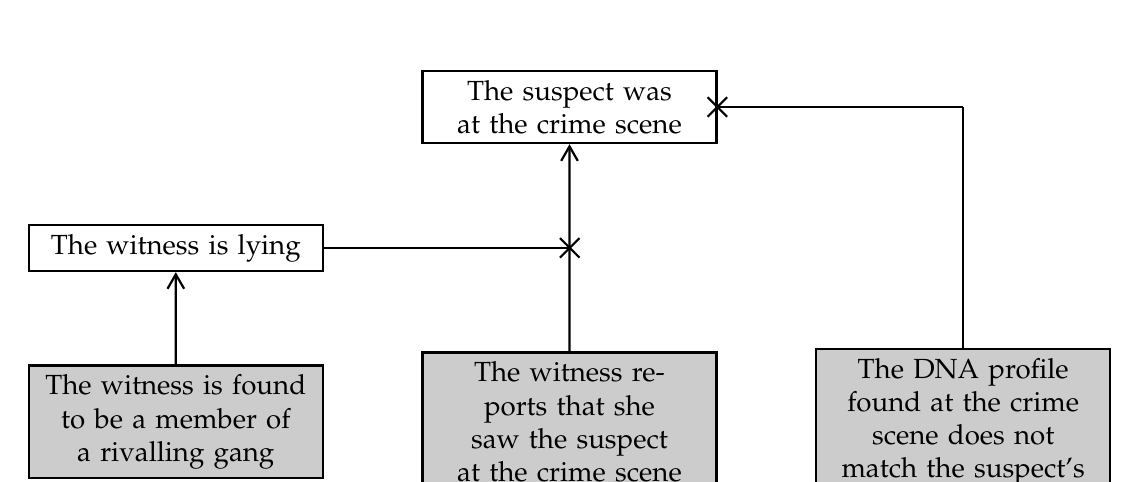
\begin{tikzpicture}[
		scnnode/.append style={text width=3cm},
		arg/.append style={text width=3.5cm},
	]
		\pgftransformxscale{5}
		\pgftransformyscale{2}

		% \draw[thick,dashed,rounded corners=1mm] (-1.45,0.45) rectangle (-0.55,-4.3);
		% \draw[thick,dashed,rounded corners=1mm] (-0.45,0.45) rectangle (0.
		% 45,-4.3);
		% \draw[thick,dashed,rounded corners=1mm] (0.55,0.45) rectangle (1.45,-4.3);

		\node[arg]     (conc) at (-1,0) {The suspect was at the crime scene};
%		\node[arg]     (oppconc) at (0,0) {The suspect was not at the crime scene};
		\node[arg,observed] (prem) at (-1,-2) {The witness reports that she saw the suspect at the crime scene};
		\node[arg,observed] (prem2) at (0,-2) {The DNA profile found at the crime scene does not match the suspect's};
		\node[arg,observed] (prem3) at (-2,-2) {The witness is found to be a member of a rivalling gang};

		\node[arg] (att) at ($(prem.north)!0.5!(conc.south)-(1,0)$) {The witness is lying};

		\draw[arg] (prem3) -- (att);
		\draw[] (prem2) -- (0,0);
		\draw[attack] (0,0) -- (conc);
		\draw[arg] (prem) -- (conc);
%		\draw[arg] (prem2) -- (oppconc);
%		\draw[attack] (prem2) -- (conc);
%		\draw[attack] (conc) -- (oppconc);
%		\draw[attack] (oppconc) -- (conc);
		\draw[attack] (att) -- ($(prem.north)!0.5!(conc.south)$);

	\end{tikzpicture}
\end{document}

\caption{Arguments with supporting and attacking reasons\label{fig:arg}}
\end{figure}

The analysis of the structure of arguments goes back to the early twentieth century when John Henry Wigmore developed his famous evidence charts~\citep{wigmore1913,wigmore1931}. The work by the New Evidence Scholarship~\citep{andersonEtal2005} continued from Wigmore's insights. Independently, and not focusing on evidence in criminal cases, the structure of arguments for and against conclusions was formalized and computationally studied by the philosopher John~\citet{pollock1987,pollock1995}. The work by Pollock stimulated an extensive literature on the formal and computational study of arguments for and against conclusions~\citep{vanEemerenEtal2014Ch11}.

\subsubsection{Probabilities}
The second normative framework for the correct handling of the evidence uses probabilities as main tool. The probability calculus is used to connect the probabilities of evidence and events, conditioned on each other. Consider for instance a trace found at the crime scene with a rare DNA profile of estimated frequency 1 in a billion. Because the profile is rare, a match is not often found accidentally. This statement can be made precise in the probability calculus. When $E$ expresses the evidence that the suspect's profile matches the trace's and $H$ that the suspect is not the source, we write:

\begin{quotation}
	$\Pr(E|H) = 1/10^9$
\end{quotation}

\noindent Here $\Pr(E|H)$ denotes the conditional probability that the suspect's profile matches the trace's, given the condition that the suspect is not the source. Conditional probabilities obey the famous Bayes' theorem:

\begin{quotation}
	$\Pr(H|E) = \dfrac{\Pr(E|H)}{\Pr(E)}\cdot\Pr(H)$
\end{quotation}

\noindent This formula shows how the posterior probability $\Pr(H|E)$ of the hypothesis given the evidence can be computed by multiplying the prior probability $\Pr(H)$ and the Bayes factor $\Pr(E|H)/\Pr(E)$.

The interest in probabilistic calculations as a tool for the good handling of the evidence has recently been stimulated by the statistics related to DNA profiling, and by some infamous miscarriages of justice that involved statistics, in particular the Lucia de Berk and Sally Clark cases~\citep{dawidEtal2011,fenton2011,schnepsColmez2013}. The interest is not new~\citep{tillers2011}, and can in fact be traced back to early forensic science in the late nineteenth century~\citep{taroniEtal1998}. To what extent probabilistic calculations have a place in courts has always been, and remains the subject of debate.\footnote{A recent instance of the debate concerns the R v T case, where the UK Court of Appeal restricted the use of Bayes' theorem in courts to cases with a solid statistical foundation such as DNA; see the 2012 special issue of Law, Probability and Risk; Vol. 4, No. 2. For a 1970s instance of the debate, see~\citet{finkelsteinFairley1970,tribe1971}.}

\subsubsection{Scenarios}
\label{sec:introScen}
The third normative framework for the correct handling of the evidence centers around scenario analysis. In a scenario, a coherent account of what may have happened in a case is made explicit. Different scenarios are contrasted, and evaluated, by considering their plausibility and by checking to what extent they match and contradict the available evidence. 

For instance, consider a murder case with two suspects: the victim's former partner and a robber. For each suspect, a scenario is considered that explains the murder:

\begin{description}
	\item S1: The victim's former partner killed the victim after a fight.
	\item S2: The robber killed the victim when caught during a robbery.	
\end{description}

\noindent When the robber confesses having killed the victim during a robbery, there is evidence contradicting scenario S1 and matching scenario S2.

Scenario analysis proves helpful when considering a complex case and its evidence. The coherent explanation of the evidence provided by a scenario can be regarded as a sense-making tool for handling cases with a large dossier. In particular, legal psychology has contributed to our knowledge about the role of scenarios in handling the evidence~\citep{bennettFeldman1981,penningtonHastie1993}. Scenarios were shown to be misleading, as experiments showed that a false scenario told in a sensible chronological order was more easily believed than a true scenario that was told in a random order. Still, the legal psychologists~\citet{wagenaarEtal1993} emphasised the usefulness of scenario analysis for the rational handling of the evidence, using the technique in their work on debunking dubious case decisions. Scenario analysis is connected with inference to the best explanation~\citep{pardoAllen2008}.

\subsection{Paper plan}

The three normative frameworks for the handling of evidence, arguments, scenarios, and probabilities, are connected to the first three of the central questions that we have discussed:

\begin{description}
	\item Question 1: How should we handle conflicting evidence?
	\item Question 2: How should we handle the strength of the evidence?
	\item Question 3: How should we coherently interpret the available evidence? 
When are we done?
\end{description}

\noindent Although---as we shall see---each of the three normative frameworks provides relevant insights for answering each of these three questions, the first question about conflicting evidence is especially closely related to the arguments framework, the second question about strength of the evidence in particular to the probabilities framework, and the third question about coherently interpreting the evidence most strongly to the scenarios framework.

In the following sections, these three questions will be discussed, consecutively, while emphasising the role of the three normative frameworks (Sections~\ref{sec:conf},~\ref{sec:str} and~\ref{sec:cohint}). The remaining two questions are less strongly connected to the normative frameworks, and are discussed in Sections~\ref{sec:intexc} and~\ref{sec:whenconv}:

\begin{description}
	\item Question 4: How should we collect, include, exclude evidence?
	\item Question 5: How should we decide about the facts given the evidence? When are we done?
\end{description}


\section{Conflicting evidence}
\label{sec:conf}
 	
\paragraph{Evidential reasoning in the law is a dialectical process involving reasons pro and con different reconstructions of the facts.} 

In many situations, it is clear what the facts and their legal interpretation are. Consider for instance a routine traffic violation such as speeding. If you are caught driving at 100 km/h, the speed limit is 50 km/h, and a police officer issues you a ticket, 
there is  little to dispute. Yet, cases that are litigated in court are typically more complicated either because the interpretation of 
the law is disputed or because there are conflicting reconstructions of the facts. 
(For disputes about matters of law, see OTHER CHAPTER IN HANDBOOK).
%; what interests us here %are conflicts concerning matters of fact.   
%One party may offer evidence that supports a certain reconstruction of the facts and the other party may bring evidence that support a radically different factual reconstruction. 
Conflicting reconstructions of the facts emerge when the two parties in a trial---the defense and the prosecutor in a criminal trial or 
the plaintiff in a civil trial---introduce evidence that support conflicting conclusions. 
For example, a witness for the prosecutor may assert she saw the defendant around the crime scene at the time of the crime, 
while the defense may introduce evidence that the genetic material found at the crime scene does not match the defendant's.
%The two pieces of evidence support different reconstructions of what happened, one piece of evidence placing the defendant at the 
%crime scene and the other undermining the inference. 
When two or more pieces of evidence support contradictory reconstructions of the facts, it can be hard 
to decide which piece of evidence to trust or which reconstruction to believe. 
%Conflicts between different items of evidence are ubiquitous in trials. %These conflicts trigger the need to have trials in the first place. 
%The point of a trial, in fact, is precisely to decide between conflicting factual reconstructions.

%and evidential reasoning play a pivotal role. 

%In order to resolve evidential and factual disagreements, 
Legal trials therefore often take the form of adversarial confrontations.  Each party is given the opportunity to make its case on the basis of the evidence she thinks important. But, 
trials are not confined to the mere presentation of the 
evidence by the interested parties. Since the parties will advance conflicting reconstructions of the facts, 
the dialectical testing of the evidence is also crucial. 
%In ordinary life, if someone makes a good argument backed up by good evidence, it can be appropriate to 
%believe her on such grounds alone. That is not the case in a trial. 
Although one party may make a strong case, backed up by good evidence, %this need not be enough. 
the other party may come up with a stronger case, backed up by even better evidence.  In the law, more often than not, reasoning toward factual 
conclusions is a dialectical process. The examination and cross examination of the evidence 
is the legal machinery that is used to identify which party has the stronger case.

The three normative frameworks for handling the evidence provide different perspectives on how to handle conflicting evidence.


\subsection{Arguments}

%\paragraph{Args are for different, possibly conflicting positions (Van Eemeren et al 2014; not specific for evidence)}

%???

In the argumentative normative framework, the handling of conflicting evidence is analyzed in terms of the arguments for and against the different positions considered,

\paragraph{The arguments for and against different positions have structure, involving complexes of reasons supporting and attacking positions.} 

Consider a crime case, where a witness reports that she saw the suspect at the crime scene. Then there is a reason supporting that the suspect indeed was at the crime scene, which in turn provides some support to the conclusion that the suspect committed the crime. This chain of supporting reasons is graphically depicted in Figure~\ref{fig:arg2}, on the left. When it is now discovered that the witness is a member of a rivalling gang, there is reason to believe that she is lying (Figure~\ref{fig:arg2}, on the right). The reason that the witness is lying attacks the argument on the left, in the sense that the witness testimony no longer provides support for the suspect being at the crime scene.

\begin{figure}[bt]
\centering
\documentclass[border=5mm,tikz]{standalone} 

\usepackage{amsmath}
% !TEX root=img/arguments_and_attack.tex

% \usetikzlibrary{external} 
% \tikzexternalize[prefix=tikz/] 

\usetikzlibrary{calc}
\usetikzlibrary{arrows}
\usetikzlibrary{arrows.meta}
\usetikzlibrary{decorations.markings}
% \usetikzlibrary{intersections}
\usetikzlibrary{fit}
\usetikzlibrary{shapes}
% \usetikzlibrary{trees}


\tikzset{
	every path/.style={thick},
	align=center,
	observed/.style={
		fill=black!20,
	},
	bn/.style={
		draw,
		ellipse,
		-{Triangle[angle=60:6pt 0]}
	},
	scn/.style={
		draw,
		rectangle,
		% signal,
		% signal from=west,
		% signal pointer angle=120,
		-{Triangle[angle=60:6pt 0]},
	},
	possibly/.style={dashed},
	arg/.style={
		draw,
		rectangle,
		-{Straight Barb[angle=60:6pt 0]}
	},
	attack/.style={
		-{Rays[width=10pt,length=10pt,sep=-3.9pt]}
	},
	pref/.style={
		draw,
		rectangle,
		-{Straight Barb[angle=60:6pt 0]}
	},
	subscn/.style={
		double,
		-{Triangle[angle=60:6pt 0]},
	},
	specific/.style={
		double,
		-{Stealth[angle=60:6pt 0]}
	},
}



\begin{document}
	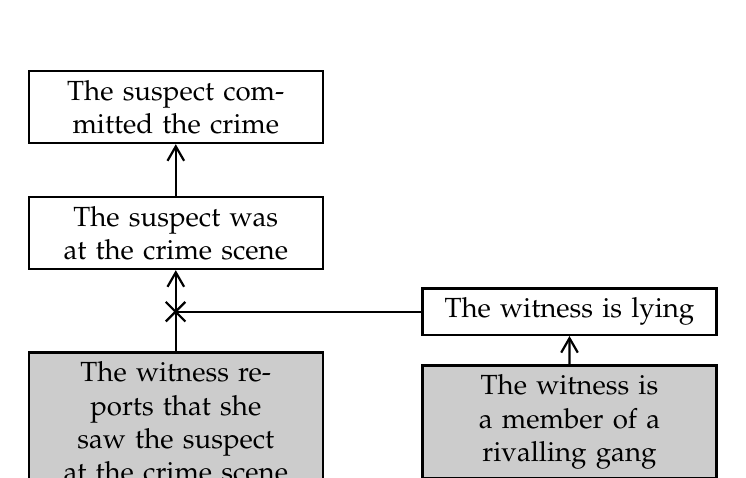
\begin{tikzpicture}[
		scnnode/.append style={text width=3cm},
		arg/.append style={text width=3.5cm},
	]
		\pgftransformxscale{5}
		\pgftransformyscale{2}

		\node[arg]     			(comm) at (0,0) {The suspect committed the crime};
		\node[arg]     			(scene) at (0,-0.8) {The suspect was at the crime scene};
		\node[arg,observed] (witn) at (0,-2) {The witness reports that she saw the suspect at the crime scene};

		\draw[arg] 					(witn) -- (scene);
		\draw[arg] 					(scene) -- (comm);

		\node[arg] 					(lying) at (1,-1.3) {The witness is lying};
		\node[arg,observed] (rival) at (1,-2) {The witness is a member of a rivalling gang};

		\draw[attack] 			(lying) -- (0, -1.3);
		\draw[arg] 					(rival) -- (lying);

	\end{tikzpicture}
\end{document}

\caption{Arguments have structure\label{fig:arg2}}
\end{figure}


\paragraph{Three kinds of attack can be distinguished: rebutting, undercutting, and undermining attack.}

Consider again the argument for the position that the suspect was at the crime scene, as supported by the reason of a witness reporting that she saw the suspect at the crime scene (Figure~\ref{fig:arg3}, on the left). This argument can be attacked in three ways. First, its conclusion can be attacked. The suspect can for instance have an alibi, showing that he was not at the crime scene. Such an attacking reason that supports an opposite conclusion is called a rebutting attack. Second, the connection between the reason and the conclusion can be attacked. The lying of the witness is an example of such an attack, referred to as an undercutting attack. In contrast with a rebutting attack, an undercutting attack provides no support for the opposite conclusion. In the example, when the witness is lying, there is no reason supporting that the suspect was not at the crime scene. Third, the reason itself can be attacked. For instance, when the witness report is fraudulent, it can be supported that the witness did not report that she saw the suspect at the crime scene. This kind of attack is referred to as undermining attack. The three examples of the different kinds of attack are shown in Figure~\ref{fig:arg3}, on the right.


\begin{figure}[bt]
\centering
\documentclass[border=5mm,tikz]{standalone} 

\usepackage{amsmath}
% !TEX root=img/arguments_and_attack.tex

% \usetikzlibrary{external} 
% \tikzexternalize[prefix=tikz/] 

\usetikzlibrary{calc}
\usetikzlibrary{arrows}
\usetikzlibrary{arrows.meta}
\usetikzlibrary{decorations.markings}
% \usetikzlibrary{intersections}
\usetikzlibrary{fit}
\usetikzlibrary{shapes}
% \usetikzlibrary{trees}


\tikzset{
	every path/.style={thick},
	align=center,
	observed/.style={
		fill=black!20,
	},
	bn/.style={
		draw,
		ellipse,
		-{Triangle[angle=60:6pt 0]}
	},
	scn/.style={
		draw,
		rectangle,
		% signal,
		% signal from=west,
		% signal pointer angle=120,
		-{Triangle[angle=60:6pt 0]},
	},
	possibly/.style={dashed},
	arg/.style={
		draw,
		rectangle,
		-{Straight Barb[angle=60:6pt 0]}
	},
	attack/.style={
		-{Rays[width=10pt,length=10pt,sep=-3.9pt]}
	},
	pref/.style={
		draw,
		rectangle,
		-{Straight Barb[angle=60:6pt 0]}
	},
	subscn/.style={
		double,
		-{Triangle[angle=60:6pt 0]},
	},
	specific/.style={
		double,
		-{Stealth[angle=60:6pt 0]}
	},
}



\begin{document}
	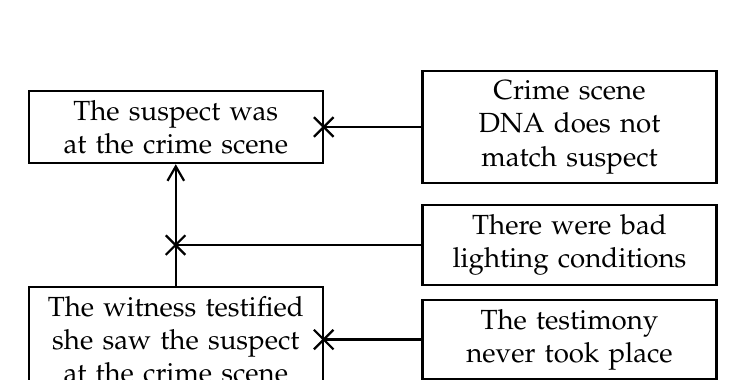
\begin{tikzpicture}[
		scnnode/.append style={text width=3cm},
		arg/.append style={text width=3.5cm},
	]
		\pgftransformxscale{5}
		\pgftransformyscale{2}

		\node[arg]     			(scene) at (0,-0.65) {The suspect was at the crime scene};
		\node[arg] (witn) at (0,-2) {The witness testified she saw the suspect at the crime scene};

		%\node[arg] 					(alibi) at (1,-0.65) {The suspect has an alibi}; 
		\node[arg] 					(alibi) at (1,-0.65) {Crime scene DNA does not match suspect}; 
		%\node[arg] 					(lying) at (1,-1.3) {The witness is lying};
		\node[arg] 					(lying) at (1,-1.4) {There were bad lighting conditions};
		\node[arg] 					(fraud) at (1,-2) {The testimony never took place};

		\draw[arg] 					(witn) -- (scene);

		\draw[attack] 			(alibi) -- (scene);
		\draw[attack] 			(lying) -- (0, -1.4);
		\draw[attack] 			(fraud) -- (witn);

	\end{tikzpicture}
\end{document}

\caption{Three kinds of attack\label{fig:arg3}}
\end{figure}

\paragraph{In an argumentative dialogue, parties take positions supported by reasons that can be challenged by attacking reasons.}

Arguments have a dialogical counterpart, in which parties exchange reasons for and against the positions they endorse. The arguments shown in Figure~\ref{fig:arg2} for instance form the backbone of the following argumentative dialogue---here presented as a fictitious, stylized discussion between judge, prosecution and defense:

\begin{description}
	\item \emph{Prosecution}: The suspect committed the crime.
	\item \emph{Judge}: Why do you believe that?
	\item \emph{Prosecution}: The suspect was at the crime scene.
	\item \emph{Judge}: Do you have evidence supporting that position?
	\item \emph{Prosecution}: There is a witness reporting that she saw the suspect at the crime scene.
	\item \emph{Defense}: Objection, your honor! The witness is lying.
	\item \emph{Judge}: Why do you believe that?
	\item \emph{Defense}: The witness is a member of a rivalling gang.
\end{description}

\noindent Models of argumentative dialogue involve specifications of the kinds of moves parties can make, the commitments these moves imply for parties, and the rules that determine the allowed sequences of dialogue moves.

\begin{comment}

\paragraph{Dialectical aspect of arguments and Argument can support a certain conclusion (i.e. premises support a conclusion)}

An argument is a collection of statements in which one statement is the conclusion and 
the others are the premises functioning as evidence for the conclusion. 
%But this definition is incomplete, for arguments can be better understood in the context of ongoing disagreements 
%between two or more parties. 
Premises and conclusions, however, are contextual notions. Consider the collection of statements $\{$I am getting wet; it is raining$\}$. Which is the premise? Which is the conclusion? 
This depends on what is at issue. If the weather condition is at issue, getting wet is the premise functioning as evidence for the conclusion 
that it is raining. If, instead, one's physical condition is at issue, the fact that it 
is raining is the premise functioning as evidence for the conclusion that one is getting wet. In this sense, the conclusion of an argument 
is what the interlocutors disagree about, while the premises 
represent what the interlocutors take as evidence that can prove or disprove the conclusion. 
\paragraph{Arguments can attack other arguments}
		
		
		
There are different ways in which two interlocutors can disagree as they put forward 
conflicting arguments. The argumentation theorist Pollock has distinguished 
two such ways, typically referred to in the literature as rebutting and undercutting  (REFERENCE). These forms of conflict between arguments 
occur in everyday discussions, but occur also in a court of law while the prosecution and defense argue a case. 

\paragraph{Rebutting: Arg2 leads to a different conclusion from Arg1}
		
		
Let us begin with \textit{rebutting}. Suppose A offers an argument for conclusion X, and B responds with an argument 
for conclusion Y, while X and Y cannot be both true, or in other words, X and Y are contradictory.  When two arguments support contradictory 
conclusions, they rebut one another. Here is a legal illustration. 
In the British case, R v Adams [1996] 2 Cr App R 467, the victim was raped and the defendant's DNA 
matched with the traces of semen found on the victim's body. %The probability that a random person would match those traces was estimated to be 1 in 200 million. But, %the victim gave a description of the perpetrator that did not match Adam's features. Second, when the victim was asked whether Adam raped her, she was unable to identify him. Finally, 
The prosecutor used the DNA match as a premise to support the conclusion that Adam raped the victim. But, Adam had an alibi---his girlfriend claimed he was with her when the crime 
occurred---and so the defense used the alibi as a premise to support the contradictory conclusion 
that Adam had nothing to do with the crime. This is an example of rebutting, because the two conclusions, each supported 
by a different piece of evidence, cannot be concurrently maintained. 

%This is an example of rebutting. 
%suggests Adam's guilt, while his alibi %, the victim's failure to recognize Adam as the perpetrator, and the fact that Adams did not match the victim's description of the perpetrator, all these pieces of information 
%points to his innocence. 
%An eyewitness claims she saw the defendant near the crime scene at the time of the crime, 
%and the defendant provides an alibi that places him far way from the crime scene at the time of the crime. 
%The statement of the witness functions as a premise for the conclusion that the defendant was around the crime scene at the time of the crime.
%The defendant's alibi, instead, functions as a premise for the (contradictory) conclusion that the defendant was \textit{not} 
%around the crime scene at the time of the crime. 

%Or, a witness claims that the criminal has blond hair, but the suspect whose DNA matched 
%that of the trace at the crime scene, has dark hair. 
%For example, A claims that it is raining outside because the streets are wet, while B claims that it is \textit{not} raining because the sun is shining. 

\paragraph{Undercutting: Arg2 attacks the relation between Premises and Conclusion in Arg1}

Turning now to \textit{undercutting}, suppose A offers an argument for X consisting in premises 
P1, P2, etc., while B shows that the premises do not support X, or at least, not as strongly as A thought. 
%This form of argument attack is known as \textit{undercutting}.
%For example, A claims that it is raining outside because the streets are wet, while B remarks that the streets are 
%wet because the sprinklers are on. B has shown that the premise `the streets are wet' 
%does not support the conclusion 'it is raining' since 
%the street got wet because of the sprinklers not the rain.
%Here is another example. A claims that it is \textit{not} raining because 
%the sun is shining, and B remarks that sometime she saw the sun shine while rain was falling.
%B has shown that the premise 'the sun is shining' does not support the conclusion `it is not raining' 
%because there are cases in which the premise is true but the conclusion false.  These are cases of \textit{undercutting}.  
%Here is an example. Premise 1: The victim was killed with a knife. Premises 2: The defendant has a cut on his hand. Conclusion: The defendant killed the victim. Premises 1 and 2, together, do lend some support to the conclusion. Yet, if we knew that the defendant had caused his cut on his hand while cooking, the premises would be undercut, in the sense that they would cease to lend any support to the conclusion. 
 Here is  an example. A prosecutor expert testifies that the defendant's 
 DNA matches the crime scene DNA, and the prosecutor uses the expert testimony as evidence 
 for the conclusion that the defendant visited the crime scene. But, suppose the expert for the defense 
 testifies that the genetic profile used for the match is shared by millions of individuals. This information undercuts, or at least significantly 
 weakens, the support that the DNA match lends to the conclusion that the defendant visited the crime scene. 

\paragraph{Undermining: Arg2 attacks the premises on which Arg1 is based}

Besides rebutting and undercutting, some argumentation theorists (REFERENCES) identify a third way in which 
two arguments can conflict. This form of conflict is sometimes called \textit{undermining}.
Suppose A offers an argument for conclusion X consisting in premises P1, P2, etc., 
while B shows that one of the premises is false. For example, given the premise that the defendant 
matches the crime scene DNA, the prosecutor argues 
that the defendant visited the crime scene. The defense, on the other hand, points out that 
a laboratory error occurred and thus alleges that the premise in the prosecutor's 
argument, namely the DNA match, is false. If the laboratory made a mistake, the DNA match declared by the laboratory  need not 
be a true match.  This is a case of undermining because one of the premises 
in the proposed argument is false, or at least this is what one party in the dispute claims.
 
\paragraph{Wigmore's charts} 
John Wigmore, as early as the beginning of the 20th century, devised a systematic method to chart arguments by identifying the
 various pieces of evidence and the relations of support and attack (REFERENCE). ILLUSTRATE REBUTTING, UNDERCUTTING AND UNDERMINING WITH WIGMORE CHARTS.
  %This becomes especially clear if we use argument charts to describe legal cases in their entirety. 
 In a court of law, the two parties in a trial aim to establish various conclusions, 
but the ultimate conclusion at issue is whether the defendant is guilty.  
The difficulty is that arguments aimed to establish the defendant's guilt can 
be intricate, and charting them with the Wigmore's method
can be extremely laborious and complicated.  SHOW A VERY COMPLEX WIGMORE CHARTS TO MAKE THE POINT THAT THEY 
  ARE OFTEN UNREADABLE AND NOT INTUITIVE. 
 Charting the arguments in a legal cases with Wigmore's charts might not be the best way to grasp a 
case as a whole. This might explain 
why, despite their clarity and precision, Wigmore's charts have 
 never been popular among lawyers and practitioners. 
 %The reason for this might be that charting arguments can often seem unnatural and needlessly complicated.
\end{comment}

  


\subsection{Scenarios}

Also the scenario perspective sheds light on the treatment of conflicting evidence. We illustrate the use of conflicting evidence in a scenario perspective by going back to the example in Section~\ref{sec:introScen}. In the example, there were three main scenarios: the breakup murder scenario $S_1$, the innocent former partner scenario $S_2$, and the caught robber scenario $S_3$ (Figure~\ref{fig:scens}).




\begin{figure}[bt]
\centering
\documentclass[border=5mm,tikz]{standalone} 

\usepackage{amsmath}
% !TEX root=img/arguments_and_attack.tex

% \usetikzlibrary{external} 
% \tikzexternalize[prefix=tikz/] 

\usetikzlibrary{calc}
\usetikzlibrary{arrows}
\usetikzlibrary{arrows.meta}
\usetikzlibrary{decorations.markings}
% \usetikzlibrary{intersections}
\usetikzlibrary{fit}
\usetikzlibrary{shapes}
% \usetikzlibrary{trees}


\tikzset{
	every path/.style={thick},
	align=center,
	observed/.style={
		fill=black!20,
	},
	bn/.style={
		draw,
		ellipse,
		-{Triangle[angle=60:6pt 0]}
	},
	scn/.style={
		draw,
		rectangle,
		% signal,
		% signal from=west,
		% signal pointer angle=120,
		-{Triangle[angle=60:6pt 0]},
	},
	possibly/.style={dashed},
	arg/.style={
		draw,
		rectangle,
		-{Straight Barb[angle=60:6pt 0]}
	},
	attack/.style={
		-{Rays[width=10pt,length=10pt,sep=-3.9pt]}
	},
	pref/.style={
		draw,
		rectangle,
		-{Straight Barb[angle=60:6pt 0]}
	},
	subscn/.style={
		double,
		-{Triangle[angle=60:6pt 0]},
	},
	specific/.style={
		double,
		-{Stealth[angle=60:6pt 0]}
	},
}



\begin{document}
	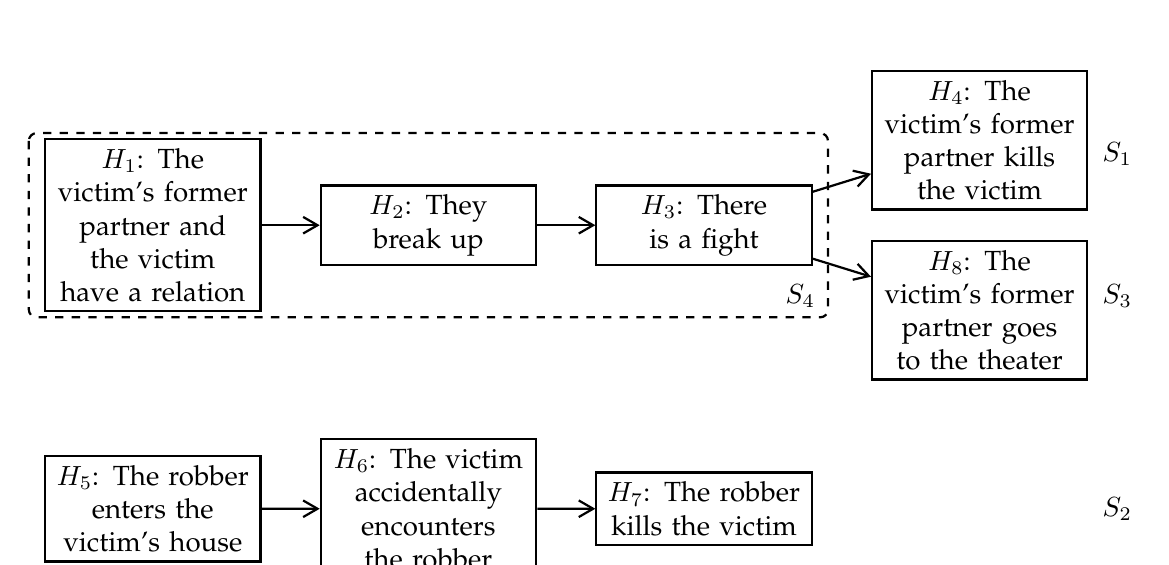
\begin{tikzpicture}[
		scn/.append style={text width=2.5cm},
		arg/.append style={text width=3cm},
	]
		\pgftransformxscale{3.5}
		\pgftransformyscale{1.8}
		
		\node[scn] (H1) at (1,0) {$H_1$: The victim's former partner and the victim have a relation};
		\node[scn] (H2) at (2,0) {$H_2$: They break up};
		\node[scn] (H3) at (3,0) {$H_3$: There is a fight};

		\node[scn] (H4) at (4,0.6) {$H_4$: The victim's former partner kills the victim};

		\node at (4.5,0.5) {$S_1$};

		\node[scn] (H8) at (4,-0.6) {$H_8$: The victim's former partner goes to the theater};

		\node at (4.5,-0.5) {$S_3$};

		\node[scn] (H5) at (1,-2) {$H_5$: The robber enters the victim's house};
		\node[scn] (H6) at (2,-2) {$H_6$: The victim accidentally encounters the robber};
		\node[scn] (H7) at (3,-2) {$H_7$: The robber kills the victim};

		\node at (4.5,-2) {$S_2$};

		\draw[thick,dashed,rounded corners=1mm] (0.55,0.65) rectangle (3.45,-0.65);
		\node at (3.35,-0.5) {$S_4$};

		\draw[arg] (H1) -- (H2);
		\draw[arg] (H2) -- (H3);
		\draw[arg] (H3) -- (H4);
		\draw[arg] (H3) -- (H8);
		\draw[arg] (H5) -- (H6);
		\draw[arg] (H6) -- (H7);


	\end{tikzpicture}
\end{document}

\caption{Scenarios\label{fig:scens}}
\end{figure}

\paragraph{Several scenarios and their relations}

In the scenario framework, it is natural to consider several mutually inconsistent scenarios simultaneously. Scenarios can have different relations with one another. They can be mutually inconsistent, such as the two murder scenarios $S_1$ and $S_3$ that each assume a different killer. They can be compatible, such as the innocent former partner scenario $S_2$ and the caught robber scenario $S_3$ that both can be true. They can have subscenario relations, such as the break up fight scenario $S_4$ (in the figure consisting of the events $H_1$, $H_2$ and $H_3$) that is a subscenario of the two scenarios $S_1$ and $S_2$ involving the victim's former partner.


\paragraph{Scenarios as alternative explanations of the evidence}

Scenarios can be considered as alternative explanations of the evidence. Returning to the three pieces of evidence discussed in Section~\ref{sec:introScen}, we see that the breakup murder scenario $S1$ explains the skin trace $E1$, the innocent former partner scenario $S2$ explains the skin trace $E1$ and the bank card use $E2$, and the caught robber scenario explains the confession $E3$.



\textbf{COPIED FROM THAT SECTION; REORGANIZE; my suggestion: that section even briefer.} the breakup murder scenario $S1$ explains the skin trace $E1$, but is contradicted by the use of the bank card $E2$, and again by the confession $E3$. The innocent former partner scenario $S2$ explains the skin trace $E1$ and the bank card use $E2$, and is independent from the confession $E3$. The caught robber scenario explains the confession $E3$, and is independent from the skin trace $E1$ and the bank card use $E2$. Considering these scenarios and this evidence, breakup murder scenario $S1$ is hard to believe, the innocent former partner and caught robber scenarios $S2$ and $S3$ seem to be true.

\paragraph{Comparative adequacy of alternative scenarios/hypotheses in explaining the evidence}





\subsection{Probabilities}

\paragraph{Evidential favoring and disfavoring can be characterized as ``probability difference''} A piece of evidence $E$ favors an 
hypothesis $H$ whenever $E$ raises the probability of $H$, or in symbols, 
$P(H|E) > P(H)$. 
For example, a witness 
testifies that she saw the defendant around the crime scene
 at the time of the crime. The testimony favors the hypothesis 
 that the defendant is guilty. 
This can be described probabilistically, as follows:
 %
 \[ P(\textit{guilt}|\textit{testimony}) > P(\textit{guilt}).\] 
 %
By contrast, a piece of evidence $E$ disfavors an hypothesis $H$ whenever $E$ lowers 
the probability of $H$, or in symbols, $P(H|E) < P(H)$.
For example, if a DNA test shows no match between the traces found at the crime
 scene and the defendant, this evidence disfavors the hypothesis that the defendant is guilty. 
 Probabilistically, 
%
\[ P(\textit{guilt}|\textit{no DNA match}) < P(\textit{guilt}).\]  
%
 %
 
% \paragraph{Two characterizations of evidential favoring and disfavoring are equivalent} 
\paragraph{Evidential favoring and disfavoring can be characterized as ``likelihood ratio''} 

There is another characterization of evidential favoring and disfavoring. 
Instead of comparing the initial probability $P(H)$ and the probability $P(H|E)$ 
of the hypothesis given the evidence, a so-called likelihood ratio of 
the form $\frac{P(E| H)}{P(E |\neg H)}$ can also be used.
On this account, $E$ favors $H$ whenever the likelihood ratio
$\frac{P(E|H)}{P(E | \neg H)}$ is greater than one. Intuitively, this means that the presence of the 
evidence is more likely if the hypothesis is true than if the hypothesis is false. 
By contrast, a piece of evidence $E$ disfavors an hypothesis $H$ whenever 
the likelihood ratio is lower than one. This means that the presence of the evidence is less likely if the 
hypothesis is true than if the hypothesis is false. In terms of the two examples considered earlier, we have:
%
 \[\frac{P(\textit{testimony}|\textit{guilt})}{P(\textit{testimony}|\neg \textit{guilt})} > 1, \text{ and }\]
 %
 \[\frac{P(\textit{no DBA match}|\textit{guilt})}{P(\textit{no DNA match}|\neg \textit{guilt})} < 1.\]
%
Interestingly enough, the two characterizations of evidential favoring/disfavoring---in terms of probability 
increase/decrease, and in terms of a likelihood ratio greater/lower than one---are 
in fact equivalent. 
For the following statements hold:
%
%\[\textit{\text{$E$ favors (or supports) $H$} iff }   P(H|E)> P(H) \textit{ iff }\frac{P(E|H)}{P(E|\neg H)}>1.\]
\[ P(H|E)> P(H) \text{ iff }\frac{P(E|H)}{P(E|\neg H)}>1.\footnote{To see why, recall that 
%
\[ \frac{P(H|E)}{P(\neg H | E)} = \frac{P(E | H)}{P(E| \neg H)}\times \frac{P(H)}{P(\neg H)},\]
%
which implies
%
\[\frac{P(E|H)}{P(E|\neg H)}>1 \text{ iff } \frac{P(H|E)}{P(\neg H | E)} > \frac{P(H)}{P(\neg H)}.\]
%
For one direction, if $P(H|E)> P(H)$, then $1- P(H|E)< 1- P(H)$. This means that 
$\frac{P(H|E)}{1- P(H | E)} > \frac{P(H)}{1- P(H)}$, and thus
$\frac{P(H|E)}{P(\neg H | E)} > \frac{P(H)}{P(\neg H)}$. So, by the equivalence above, $\frac{P(E|H)}{P(E|\neg H)}>1$.
For the other direction, if $\frac{P(E|H)}{P(E|\neg H)}>1$, then $\frac{P(H|E)}{P(\neg H | E)} > \frac{P(H)}{P(\neg H)}$, again 
by the equivalence above. 
The latter is the same as $\frac{P(H|E)}{1- P(H | E)} > \frac{P(H)}{1- P(H)}$. To establish $P(H|E)> P(H)$, suppose for contradiction that
$P(H|E) \leq P(H)$, which implies $1- P(H|E) \geq 1- P(H)$. This means that $\frac{P(H|E)}{1- P(H | E)} \leq \frac{P(H)}{1- P(H)}$. 
This contradicts $\frac{P(H|E)}{1- P(H | E)} > \frac{P(H)}{1- P(H)}$, and thus $P(H|E)> P(H)$.}\]
 %
\[ P(H|E) < P(H) \text{ iff}  \frac{P(E|H)}{P(E|\neg H)} < 1.\]
%

\paragraph{The conflict between two pieces of evidence can be described probabilistically}
Two pieces of evidence come into 
conflict with one another insofar as one favors an hypothesis 
and the other disfavors the same hypothesis. 
The conflict can be described probabilistically, in that one piece of evidence increases 
the probability of the hypothesis, while the other decreases it, or equivalently, the likelihood ratio is positive (for one piece 
of evidence) and negative (for the other). 
For example, the testimony that the defendant was around the crime scene conflicts 
with the lack of a DNA match. Probabilistically, the testimony 
increases the probability of the defendant's guilt (or equivalently, the likelihood ratio is greater than one),
while the lack of a DNA match decreases the probability of the same hypothesis 
(or equivalently, the likelihood ratio is lower than one).







\subsection{Further reading}

Arguments: Wigmore, references Pollock 1995, Dung 1995; ?mention nonmonlog, Toulmin's anti-logicism, FvE/Walton


\section{Evidential Value}
\label{sec:str}

\subsection{Probability}



\paragraph{Evidential value can be quantified as probability difference, likelihood ratio or overall probability}
The value of the evidence for, or against, an hypothesis 
can be quantified probabilistically in various ways. 
%The probabilistic framework allows us to quantify the strength of the evidential favoring or support relation between evidence and hypothesis. 
%The are different approaches in the literature. % (FITELSON REFERENCE HERE). 
%Let us begin with quantifying the value of the evidence \textit{for} an hypothesis. 
One approach considers the difference between the probability of 
the hypothesis with and without the evidence, that is, $P(H | E) - P(H)$.
%If $P(H | E)$ is higher than $P(H)$, this means that the evidence lends some support to
%the hypothesis. 
The larger the positive difference, the higher the value of the evidence 
for the hypothesis. 
%By contrast, the larger the negative difference, the higher the value of the evidence against the hypothesis. 
An alternative approach is given by the likelihood ratio $\frac{P(E|H)}{P(E| \neg H)}$. 
%For the evidence to offer some support to the hypothesis, the likelihood ratio should be at least greater than one. 
For any value greater than one, the higher the likelihood ratio, 
the higher the value of the evidence for the hypothesis. %For simplicity, we shall speak of evidential strength 
%in terms of likelihood ratios, as follows:
%
%\begin{quote}
%\textsc{Evidential strength:} The evidential strength of $E$ relative to $H$ is proportional to 
%the likelihood ratio $\frac{P(H|E)}{P(H|\neg E)}$. 
%\end{quote}
%
%By contrast, for any value lower than one, the lower the likelihood ratio 
%the higher value of the evidence against the hypothesis. 
\begin{comment} 
The following table %, whose calculations are approximations based on Bayes' theorem, offers 
offers some illustrations:

\vspace{2mm}
\hspace{0.5cm}
\begin{centering}
\begin{tabular}{lccccc}
\hline
$P(H)$ & Likelihood Ratio & $P(H | E)$ &  $P(H|E)-P(H)$ \\
\hline
0.0001 & 1,000 & 0.09 &  0.0899   \\
%0.001 & 1,000 & 0.049 & 0.5  \\
%0.01  & 1,000 & 0.08  & 0.9 \\
0.1 & 1,000  & 0.99 &  0.89 \\
\hline
%0.5 & 1,000 &   0.999 \\
%0.9 & 1,000 &   0.9999 \\
0.0001 & 10  & 0.001 &  0.0009 \\
0.01 & 10  & 0.09 &  0.08  \\
\hline
\end{tabular}
\end{centering}
\vspace{2mm}

\noindent
%Note that even if the likelihood ratio is high, the probability $P(G|E)$ can 
%still be low if the initial probability $P(H)$ is itself low. 
All in all, a positive difference $P(H|E) - P(H)$ and a likelihood ratio $\frac{P(E|H)}{P(E| \neg H)}$ greater than one
%tell us how much a piece of evidence $E$ can impact upwards the initial 
%probability of a hypothesis $H$. They 
quantify, albeit in different ways, the value of the evidence \textit{for} 
an hypothesis. 
\end{comment}
 By contrast, a negative difference $P(H | E) - P(H)$ and a likelihood ratio lower than one  
quantify the value of the evidence \textit{against} an hypothesis.
The larger the negative difference and the lower the likelihood ratio (for any value below one), 
the higher the value of the evidence against the hypothesis.

%As one can see from the table, there are quantitive 
%differences between the two approaches, but these should 
%not concern us here. Since the most widely used approach to quantify evidential value relies on 
%likelihood ratios, we shall use that, making occasional 
%references to the other approach if necessary. 

%\paragraph{The overall probability is not the same as probability difference and likelihood ratio}

Intuitively, the value of a piece of evidence for or against an hypothesis can also be quantified by the probability 
of the hypothesis given the evidence. The higher, or lower, the probability $P(H|E)$, the higher 
the value of the evidence for, or against, the hypothesis. The probability $P(H|E)$, however, should not be confused with the probability difference or the likelihood ratio. To illustrate, suppose a witness testifies that the defendant beat the victim to death, but as it turns out, the witness 
was drunk at the time, so the evidential value of the testimony in favor of guilt is low. 
If the testimony by the drunk witness is the only incriminating evidence, the probability 
$P(\textit{guilt} | \textit{drunk witness})$ should also be low. Now, it follows that $P(\textit{innocence} | \textit{drunk witness})$ 
should be high insofar as \textit{innocence} is the negation of \textit{guilt}. 
But this seems problematic. A drunk witness, in fact, is of little help in establishing 
innocence (just as it is of little help in establishing guilt).

It is instructive to quantify the value of the testimony in favor of guilt by means of 
the probability difference and the likelihood ratio. Since the witness was drunk, the value of the evidence in favor of guilt is 
low, that is:
%
\[\text{the positive difference $P(\textit{guilt} | \textit{drunk witness}) - P(\textit{guilt})$ is small, and}\]
%
%
\[\text{the likelihood ratio $\frac{P(\textit{guilt} | \textit{drunk witness})}{P(\textit{guilt} | \neg\textit{drunk witness})}$ is only slightly above one}.\] 
%
Similarly, the value of the evidence in favor of innocence is also low, that is:
%
\[\text{the negative difference $P(\textit{innocence} | \textit{drunk witness}) - P(\textit{guilt})$ is small, and}\]
%
%
\[\text{the likelihood ratio $\frac{P(\textit{innocence} | \textit{drunk witness})}{P(\textit{innocence} | \neg\textit{drunk witness})}$ is only slightly below one}.\] 
%
So, the value of the testimony in favor of guilt, and innocence, is low 
in both cases. This means that $P(\textit{guilt} | \textit{drunk witness})$
and $P(\textit{guilt})$ are roughly the same value, and so are $P(\textit{innocence} | \textit{drunk witness})$ 
and $P(\textit{innocence})$. Consequently, if $P(\textit{innocence})$ is high, 
and thus $P(\textit{guilt})$ low, $P(\textit{innocence} | \textit{drunk witness})$ will 
be high, and thus $P(\textit{guilt} | \textit{drunk witness})$ low. %, given the little evidential value of the testimony. 
We should thus not be surprised that $P(\textit{innocence} | \textit{drunk witness})$ is high. 
This is because, by Bayes' theorem, $P(H|E)$ depends on $P(H)$.  
Even if $E$ does not change significantly the probability of $H$, or the likelihood ratio (positive or negative) 
$\frac{P(E|H)}{P(E| \neg H)}$ is small, $P(H|E)$ could still be high or low, insofar as $P(H)$ itself is high or low. 
All in all, we should be careful in not confusing a high probability $P(H|E)$ with a high 
evidential value in terms of a large probability difference or a high likelihood ratio.


\paragraph{Likelihood ratio can quantify the value of DNA evidence}



The most widely used measure of evidential value 
is the likelihood ratio. As an illustration, let us determine the likelihood ratio 
of a DNA match in favor of guilt. %, where the match is between
%the crime scene's genetic profile and the defendant's. 
First, it is important to realize that the hypothesis of guilt is not equivalent to 
other propositions, such as the following: %which are progressively more removed from guilt: 

- the \textit{lab reports} that the defendant's 
genetic profile matches with the crime traces;

- the defendant's genetic profile \textit{truly matches} with the crime traces; 

- the defendant is the \textit{source} of the traces; and

%the defendant \textit{left} the crime traces; 

%the defendant \textit{visited} the crime scene; 

%the defendant \textit{participated} in the crime; 

- the defendant is \textit{guilty}.

\noindent
The inference from `reported match'  
to `guilt', passing though the intermediate steps `true match' and 'source', is a complex one, 
and many sources of error may undermine the inference along the way.  
To ease exposition, we make three simplifying 
assumptions. The first is that the inference from `reported match' to `true match' is unobjectionable, or in other words, we assume that 
the DNA test reporting a match (or a non-match) is infallible. This, of course, need be the case because laboratories make mistakes.
The second assumption concerns the inference from `true match' to `source'.
Even if one is a true match, one need not be the source. A genetically identical twin or someone else 
who just so happens to have an identical DNA could be the source. 
%t could also be that synthetic genetic material, perfectly matching one's DNA, was planted. 
Now, the second simplifying 
assumption is that the inference from `true match' to `source' can be undermined by 
one source of error only, namely the possibility that another individual 
could coincidentally match. This possibility is expresses through the so-called 
Random Match Probability, that is, the probability that a random person would match. 
%If RMP equal 1 in 200, we would expected 1 such profile every two hundred people or the RMP equals 0.5\%. 
Other sources of error---for example, a twin brother or an artificially synthesized DNA could be the source---will be disregard. 
%We should bear in mind that genetic profiles are not unique. Based on statistical and genetic modeling, a profile is expected to occur with a frequency in a select population. 
Finally, the third  simplifying assumption is that whoever is the source of the crime traces must be the perpetrator, 
so `guilt' and `source' are treated as equivalent. 
 This, of course, need not be the case. One could be the source of the traces without participating in the crime because, for example, 
 one visited the crime scene before or after 
 the crime took place.
 

Suppose now that the DNA test reports a match between the crime 
traces and the defendant.  Given our simplifying assumptions, 
the evidential value of the DNA match in favor of guilt, in terms of a likelihood ratio, 
is as follows % \citep{Dawid02, Balding2005Weight}:
%
\[
{P(M | G) \over P(M | \neg G)} =   {1 \over RMP}.
\]
%
If the RMP is 1 in 200 million, the likelihood ratio would be
%
\[\frac{P(M |G)}{P( M | \neg G)}=\frac{1}{\frac{1}{\text{200 million}}}=\text{200 million}.\]
%
The numerator $P(M | G)$ equal 1 because of our simplifying assumption that 'source' and guilt' are interchangeable 
and the laboratory test is infallible. If the defendant is guilty and thus the source of the crime traces, the infallible 
lab test must report a match. As for the denominator, 
%keep in mind that $RMP$ is the probability that a random person, 
%unrelated to the crime or the defendant, would be found to have a matching DNA. 
putting $P(M | \neg G)=RMP$ is plausible because (1) the probability that a match would be reported assuming that the defendant was \textit{not} 
the source is roughly the same as the chance that a random person---someone who had no contact with the victim---would match anyway, 
and because (2) 'source' and 'guilt' are, by assumption, equivalent.


%To quantify the evidential value in terms of probability difference, 
%the initial probability $P(G)$ must be known. So, as often done in the literature, it is 
%more convenient to focus on likelihood ratios.

Since the likelihood ratio in question is a high number, the DNA match in favor of guilt 
has a high evidential value. We should not forget, however, 
our simplifying assumptions. For example, a likelihood ratio as high as 
1 billion reduces to about 100 if the laboratory error rate is 1\% \citep{Thomason2003How-the-Probabi}.
%More generally, the fallibility of a DNA test has negative impact on the value of the evidence insofar as a higher 
%value in the denominator results in a lower likelihood ratio. 
Also, the identification of 'source' and 
`guilt' must also be taken into account, and relaxing this identification 
further weakens the value of a DNA match in favor of guilt.




\paragraph{Further readings} Lab errors for DNA evidence, see \citep{Thomason2003How-the-Probabi}, 
\citep{Buckleton2005A-Framework-for}. Prosecutor fallacy \citep{Thompson1987Interpretation}. The fact the a match 
is not a all-or-nothing affair \citep{Kaye1993Dna}. Uniqueness of DNA profiles  \citep{Buckleton2005Population, Weir2007rarity}.
Comparison between DNA evidence and fingerprint  \citep{Zabell2005Fingerprint-Evi}. Probabilistic analysis of eyewitness testimony XXX. 
Different way to formulate the likelihood ratio for DNA evidence \citep{Robertson1995DNA-Evidence:-W}
Probabilistic analyses of DNA evidence  \citep{Dawid02, Balding2005Weight}. Different hypotheses Koheler, Everett
How DNA evidence can be synthesized and implanted XXX. 



\subsection{Arguments}

\paragraph{Difference between deductive and presumptive arguments [inductive, abductive, ampliative, defeasible; what have you]}

Deductive arguments, when valid, ensure that the truth of the conclusion necessarily follows from the truth of the premises. 
Indeed, the premises might be altogether false, but in so far as they are true, 
the conclusion must unquestionably be true. Arguments in a court of law, however, can hardly be of this sort. If a witness asserts that she saw the defendant on 5th Avenue, the assertion does not establish, unquestionably, that the defendant was in fact on 5th Avenue. The argument `the witness asserts $p$, \textit{therefore} $p$' is not deductively valid. At the same time, the argument is not a worthless either, and there are two ways to see this. First, if a witness asserts that $p$ is the case, the assertion establishes---at least tentatively, \textit{prima facie}, absent contrary evidence---the truth of $p$. Second, if a witness asserts that $p$ is the case, the assertion establishes---with a high probability---the truth of $p$ (at least, provided the witness is a reliable one). In the former case, we speak of defeasibly valid arguments, and in the latter case we speak of inductively valid arguments. REFERENCE. Both types must be distinguished from deductively valid arguments in which the truth of the premises guarantees---with no exception whatsoever---the truth of the conclusion. In defeasibly or inductively valid arguments, instead, it is still possible for the conclusion to be false and the premises true. 

Defeasible or inductive 
arguments can always be transformed in deductive 
ones by adding the appropriate premises. For example, 
the defeasibly valid argument
%
\begin{quote}
The witness asserts $p$

------------------------------

Therefore, $p$
\end{quote}
%
can be rewritten as the deductively valid argument 
%
\begin{quote}
The witness asserts $p$

(+) There is no contrary evidence 

(++) Absent contrary evidence, what a witness asserts is true 

-------------------------------------------------------------------------------------------------

Therefore, $p$
\end{quote}
%
%Insofar as we are interested in whether the conclusion holds, both versions are not very different. The conclusion $p$ can be attacked, either by undercutting the connecting between the premise and the conclusion (in the defeasible/inductive version) or by undermining the premises (in the deductive version).
In the deductive version, the weaknesses of the inductive argument are explicitly laid out. It is therefore instructive to rewrite an inductive argument in the deductively valid form, so that the ways in which the inductive argument could go wrong are made explicit.  REFERENCES. 

\paragraph{Strength} In assessing the strength of arguments, two factors must be considered. The first is how strongly the premises support the conclusion. In this respect, deductively valid arguments have maximal strength because the premises unquestionably support the conclusion. But, as seen earlier, any argument can be turned into a deductively valid argument by adding the appropriate premises. This cannot mean, however, that any argument can be turned into an argument with maximal strength; this would be absurd. The strength of an argument---and this is the second factor to consider---must therefore also depend on whether the premises are well supported. We consider a number of approaches to make these ideas more precise. 


\paragraph{Args are good when surviving scrutiny under critical questions (arg schemes; Walton et al ...)}

Critical questions can be used to assess the strength of an argument. They can attack the premises, the inferential link between premises and conclusion or the conclusion itself. Of course, in a deductively valid argument, only the premises and the conclusion can be attacked, 
while in a defeasibly valid argument the inferential link between premises and conclusion 
can also be attacked. 

Consider first a defeasibly or inductively valid 
argument based on eyewitness testimony:
%
\begin{quote}
The witness asserts she saw the defendant run away from the crime scene.

---------------------------------------------------------------------------------------------------

The defendant run away from the crime scene.
\end{quote}
%
The critical questions that attack the inferential link between premise and conclusion can include: Were the visibility conditions good at the time? Does the witness have good memory? The critical questions that directly attack the conclusion itself can include: Was the defendant physically able to run away? Was defendant with his girlfriend when, allegedly, he run away from the crime scene? Critical questions are pointers toward potential counterarguments. If the questions target the inferential link, they are pointers to undercutting arguments, and if they target the conclusion itself, they are pointers to rebutting arguments. 

In the above argument, it would be pointless to formulate a critical question that attacks the premise 
itself. If the witness is speaking in court, the assertion cannot be questioned. Consider now an argument
 based on expert option:
  %
\begin{quote}
The expert asserts that Benedict intake during pregnancy causes birth defects among animals.

Benedict's effects on animals are sufficiently similar to its effects on humans.

------------------------------------------------------------------------------------------------------
 
Benedict intake during pregnancy causes birth defects in humans. REFERENCE SUPREME COURT CASE ON THAT, DAUBERT
\end{quote}
%
The critical questions targeting the inferential link here include: Is the expert competent in the domain? Is the expert credible? Is the expert reliable? Does the expert agree with other experts? REFERENCE Other questions can be used to attack the premises themselves. To be sure, it is hard to attack the first premise because the statement was presumably made in court. Still, the second premise can be doubted. Does 
Benedict affect animals and humans in the same way?  What if animals and humans react very differently? Don't animal and humans have very different digestive apaarrati?

Depending on the domain, more specific questions can be used, attacking the premises, the inferential link or the conclusion. If an expert testifies about a DNA match, the appropriate critical questions will also include: Could the match be coincidental? Did the expert comply with the laboratory protocols? Could the DNA material have been implanted?  Does the DNA match have anything to do with the guilt of the defendant? And so on. In section REFERENCE TO EARLIER SECTION, we identified different sources of uncertainty for DNA evidence. These sources correspond to specific critical questions that can be posed for expert opinions about a DNA match.  

The more critical questions an argument survives, the stronger the argument. It is not easy to say what it takes for an argument to \textit{survive} critical questions. First recall that, as noted earlier, critical questions are pointers toward a variety of counterarguments. A critical question that challenges the inferential link between premises and conclusion is a pointer to a potentially undercutting argument. A critical question that challenges one of the premises is a pointer to a potentially undermining argument. A critical questions that is directed against the conclusion itself is a pointer to a potentially rebutting argument. Given the parallelism between types of critical questions and types of attacks, 
to survive a critical question just means to survive an attack by a counterargument. To clarify this, in what follows, we shall look more closely at systems of arguments in which arguments attack and counterattack one another. REFERENCE The notion of attack and counterattack 
will be taken to be primitive. We shall next examine the notion of attack and counterattack more closely and 
offer a theory of when attack or counterattack is successful. REFERENCE

%(Some complications about critical questions. Suppose an eyewitness testifies that she saw the defendant run away from the crime scene. The defense may then ask the critical question, what were the lighting conditions at the time? If the witness answers that it was dark, this will weaken the testimony and defeat the corresponding argument based on it. If, however, the witness answers that the light was bright, this would be an adequate response. But, of course, things are not always so clear.  Suppose an expert witness testifies that the defendant matches with the DNA found on the victim's body. The defense may now ask the critical question, what if the DNA material was framed? The prosecution could simply respond that no evidence of framing was found. Would this be an adequate response? If the expectation is that the prosecution, in answering the critical question, should provide a full-fledged argument that that there was no framing, the prosecutor's response would be inadequate, and thus the argument would not survive the critical question. If, instead, the expectation is that the defense, in asking the critical question, should also provide \textit{prima facie} evidence that there was framing, the prosecutor's answer  (absent evidence to the contrary) would be adequate, and thus the argument would survive the critical question. All in all, whether an argument survives a critical question depends on whether the burden of answering the question rests entirely on the party to whom the question is addressed or whether the party who asks the question bears the burden to provide some \textit{prima facie} evidence that gives initial credibly to the question itself, and once this burden is met, the other party has the burden to provide a full-fledged argument in response. MORE EXPLANATION NEEDED. REFERENCES? SARTOR AND PRAKKEN?)

%(The allocation of burdens is sometimes explicitly regulated by law. For example, the Daubert decision mandates that the party who wishes to introduce expert opinion should qualify the opinion as meeting the requirement of reliability and competence, or else the opinion would not be admissible. The law is not always so clear, however.  For example, nowhere the law says that the prosecutor should answer questions about the lighting conditions or the memory of a witness.  In criminal trials, at least, we know that the burden of proof lies entirely with the prosecutor. We could interpret this as requiting that the prosecutor answer all critical questions with full fledged-arguments. But, it would be unreasonable to expect a prosecutor to answer \textit{all} critical questions. They can be potentially infinite, and such an expectation would make the task impossible for any prosecutor. To be sure, the law says that the prosecutor should establish the charges beyond a reasonable doubt. We can interpret this as requiring, among others things, that the prosecutor answer all critical questions that are reasonable. But this raises another question. What counts as a reasonable critical question as opposed to an unreasonable one? LITERATURE ON THE TOPIC?)


\paragraph{Args win when they can defend themselves against attacks (Dung 1995)}

Dung REFERENCE provided an abstract framework to analyze 
systems of arguments. The notion of an argument attacking another argument 
is taken as primitive. We can think of systems of argument as an alliance of arguments, and in particular, 
following Dung's framework, the system $S$ of arguments is a \textit{successful alliance} provided:
%
\begin{quote}
(\textit{conflict-free}) each argument in $S$ is not attacked by any argument in $S$; and 

(\textit{defense}) for any argument (outside $S$) that attacks any argument in $S$, there is an argument inside $S$ that attacks the attacker.
\end{quote}
%
So, a system of arguments forms a successful alliance provided there is no internal conflict and any external attack 
can be counterattacked by arguments within the alliance. The notions of a winning and losing argument can now be defined:
%
\begin{quote}
(\textit{winning})  $A$ \textit{wins} provided $A$ is part of a successful alliance; and 

(\textit{losing} ) $A$ \textit{loses} provided another argument $A'$ attacks $A$ and $A'$ wins. 
\end{quote}
%
These definitions are intuitive. If an argument can defend itself from any attack by appealing to its allies, it wins. If, instead, there is a winning argument that attacks an argument, the latter loses. A problem here, however, is that an argument can be both winning and losing. 
Consider four arguments $A, B$ and $A', B'$ such that $A'$ attacks $A$ and vice versa, and $B$ attacks $B'$ and vice versa. The system $\{A, B\}$ is a successful alliance because there are no internal conflicts and any attack against $A$ or $B$ is counterattacked within the alliance $\{A, B\}$. It follows that arguments $A$ and $B$  both win. At the same time, the system $\{ A', B'\}$ is also 
a successful alliance, so arguments $A'$ and $B'$ win. This means that $A$ and $B$ both lose because each is attacked by a winning argument, and the same holds for $A'$ and $B'$.

%(Intuitively, alliance $\{A, B\}$ and $\{A', B'\}$ are symmetrical in the sense that any argument in one alliance is attacked but an argument in the other alliance. No one appears to be stronger then the other. If, however, we compared $\{A, B, C\}$ and $\{A', B'\}$ and added the condition that $C$ attacks either $A'$ or $B'$ and $\{A, B, C\}$ had no internal conflicts, it would follow that $\{A', B'\}$ is not a successful alliance anymore and thus the only winning arguments would be $A$ and $B$. One easy fix could be to require that successful alliances cannot be symmetrical to other successful alliance. This means for any give set of arguments there is only one successful alliances.)

(As far as evidential reasoning in the law is concerned, something is unsettling about this state of affairs. There is something unnatural about the systems $\{A, B\}$ and $\{A', B'\}$ and the fact that $A$ attack $A'$ and vice versa, and the same holds for $B$ and $B'$.
Suppose an eyewitness asserts she saw the defendant stab the victim and another witness asserts the eyewitness is biased because she has reasons to hate the defendant. The second witness attacks the testimony of the eyewitness. This exemplifies an attack against $A$ by $A'$. There is nothing problematic about that. But now suppose the eyewitness defended herself against the second witness by asserting that the second witness is biased against her because the witness has reasons to hate her. This exemplifies a situation in which $A$ attacks $A'$. There is nothing problematic about that either. But, although the fact that $A$ attacks $A'$ and vice versa are fine as isolated attacks, when they are considered together, they become  problematic. Suppose we engage in a conversation in which I assert conclusion $C$ on the basis of evidence $e$  and you challenge me by challenging $e$ on the basis of other evidence $e'$. Next, I defend myself by challenging your evidence $e'$ and I do so by using my evidence $e$.  You challenge targets $e$ on the basis of $e'$ and I target $e'$ on the basis of $e$. This is a stale mate and a circle of attack and counterattack. Ideally, we would need further evidence, besides $e$ and $e'$, to resolve the controversy. In the court example,  a third witness is needed who can tell us whether the first eyewitness or the second witness is biased. So, an easy fix to the above problem, especially when it comes to evidential reasoning in the law, is to require that stalemate situations or circles of attacks and counterattacks be avoided.)

\paragraph{Args win when they are better/stronger than/preferred over conflicting args}

Dung's framework considers system of arguments and the relations of attack and counterattack among arguments, but does not examine the internal structure of arguments. The notions of attack and counterattack are left unspecified, and the notion of a successful 
attack is also left unspecified. To be sure, all we can say from Dung's framework is that an attack is successful when 
it consists of a winning argument. We are told nothing more about the internal structure of arguments.

 Prakken REFERENCE has provided a unified theory of argumentation which builds on Dung's insights but also examines 
 the internal structure of arguments. As seen earlier, argument can be attacked in three ways. An argument can be attacked by offering another argument with the opposite conclusion (rebutting). An argument can be attacked by offering an argument that weakens the inferential link between premises and conclusion (undercutting). An argument can be attacked by challenging its premises (undermining). The remaining question is, when is an attack successful? 

Let us begin with an example of one argument rebutting another.  A witness asserts that the defendant stabbed the victim, while DNA evidence shows no match between the defendant and the crime traces. The argument based on an witness statements is rebutted by---but also rebuts---the argument based on the DNA match. The attack works in both direction in the sense that bother arguments attack one another regardless of which argument is made first. Is the attack successful? In Dung's framework, the answer is that both arguments win and both arguments lose (provided both arguments are part of a successful alliance). This is hardly satisfying. 

A step forward is a ranking among arguments. A rebutting argument $A'$ is considered a successful attack  on an argument $A$ whenver $A$ is ranked higher than $A'$.  How can arguments be ranked? The ranking will depend on the relative strength we assign to the premises and to the inferential link between premises and conclusion. Consider an abstract example. The first argument consists of premises $A$ and the defeasible inference $A\Rightarrow B$, while the second argument consists of premises $A'$ and the defeasible inference $A'\Rightarrow \neg B$. The conclusion of the first argument is $B$ and the conclusion of the second argument is the negation of $B$. Which argument ranks higher? This will depend on whether we consider $A$ a better premise---for example, more probable---than $A'$. It will also depend on whether we consider $A\Rightarrow B$ a better inference---for example, more likely to preserve the truth---than $A'\Rightarrow \neg B$. Clearly, other things being equal, if $A$ is better than $A'$, the first argument is ranked higher. However, if $A$ is a better premise but $A'\Rightarrow \neg B$ is a better inference, it is not easy to adjudicate the ranking of the two arguments.

Consider now a case in which an argument undercuts another argument. There is nothing peculiar about this case. We can apply the same ideas as in the rebutting case. In order for the attack to be successful, the undercutting argument must be ranked higher than the attacked argument. 
If not, the attack launched by the undercutting argument must fail. 
 
Finally, the third type of attack: undermining. An attack against a premise can consists in a one line statement that the premise is false or can be a more elaborate argument resulting in the denial of the premise. How can we tell which attacks on the premises are successful? At first blush, one mighty say that the mere statement that the premise is false would not do, but this would be too simplistic.  Premises come in different guises and sometimes it might be enough to merely disagree with a premise and some other times a more sustained argument might be necessary. To illustrate, consider three types of premises. REFERENCES TO PRAKKEN AND GORDON

First, premises can be axioms or self evident statements. If the premises are axioms or self evident, they cannot be attacked. An attack against an axiom or a self evident premise will therefore always fail. 

Second, premises can also be assumptions or statements that are taken for granted without explicitly supporting reasons. Assumptions are peculiar in that that they hold until contrary evidence shows they are false. Assumptions are close to what in the law are known as presumptions. Suppose the prosecutor argues that a mail package containing drugs was received by the defendant. The prosecutor has proof that the package was mailed and that it reached the defendant's address. The prosecutor has no explicitly proof that the packed was delivered to the defendant. The prosecutor \textit{assumes} that if the package was sent and received at the defendant's address, it was the defendant who received it. What if the defendant challenges the assumption alleging that he was not at home when the package was delivered? This raises the question of who has the burden of proof. Should the prosecutor give evidence that the assumption is correct or should the defendant give evidence that the assumption is incorrect, and in absence of contrary evidence, should the assumption be taken to be correct? 
If we are in fact dealing with an assumption, it is up to the party who challenges the assumption to show that it is correct. Assumptions are true until contrary evidence is provided. 

Finally, we have ordinary premises. These must be defended with adequate evidence and arguments and cannot be assumed the be true. If the a party attacks an argument by challenging an ordinary premise, the burden of proof is on the party proposing the argument to back up the premise. Ordinary premises, in this sense, are very different from assumptions. In short, axioms or self evident premises cannot be challenged. Assumptions are assumed to hold until contrary evidence is presented. The burden of proof is on the attacking party. Ordinary premises can only be believed on the basis of supporting evidence or arguments. The burden of prof here is on the attacked party. 

An attack against the premises of an argument will succeed or fail depending on the targeted premises. Attacks against self evident premises always fail. Attacks against assumptions are successful only if evidence is introduced that the assumption is indeed false. Attacks against ordinary premises succeeds even though no evidence that the premise is false is introduced and provided that the other party has introduced no evidence for the truth of the premise. If the other party has introduced evidence for the truth of the premise, the premise is the conclusion of an argument, and thus the attack must take form of a rebuttal.







 





 

 


\paragraph{Pros and cons can be weighed (accrual)}

\paragraph{(Mention ?Pollock's anti-probabilism)}

\subsection{Scenarios}


\section{Coherently interpreting the evidence}
\label{sec:cohint}

\subsection{Scenarios}




\paragraph{	Good properties of scenarios: completeness, plausibility (here??), coverage (see Pennington and Hastie)}

\paragraph{	Scenario schemes (Schank, Bex)}

\subsection{Arguments}

\paragraph{Inference to the best explanation (Allen/Pardo?)}

\paragraph{WORRY: Confused about this one; why is it under coherence?) [Answer BV: Otherwise nothing remains here. ]}

\subsection{Probability}


\paragraph{Independent items of evidence can be combined by multiplying the likelihood ratios}

In a criminal case, there may more than one piece of evidence, for example, 
there may be an eyewitness testimony and a DNA match. 
Suppose $P(\textit{guilt}| \textit{testimony})=0.7$
and $P(\textit{guilt} | \textit{match})=0.7$. What is the probability 
$P(\textit{guilt}| \textit{testimony} \wedge \textit{match})$ resulting 
from combing the two pieces of evidence? It would be a mistake to say that, assuming that 
the two items of evidence are independent, $P(\textit{guilt}| \textit{match} \wedge \textit{testimony})$ equals 
$0.7\times 0.7=0.49$. %How can  $P(\textit{guilt}| \textit{match}, \textit{testimony})$ be lower than  
%$P(\textit{guilt}| \textit{testimony})$ or $P(\textit{guilt}| \textit{match})$? 
The combination of two pieces of evidence, each favoring guilt to some extent, should strengthen the case for guilt, 
not weaken it. Observe that 
 %
\[\frac{P(\textit{guilt} | \textit{match}\wedge \textit{testimony})}{P(\neg \textit{guilt} | \textit{match}\wedge \textit{testimony})}=\frac{P(\textit{match}\wedge \textit{testimony} | \textit{guilt})}{P(\textit{match}\wedge \textit{testimony} | \neg \textit{guilt})}\times \frac{P(\textit{guilt})}{P(\neg \textit{guilt})},\]
 %
 and if \textit{match} and \textit{testimony} are independent, conditional on \textit{guilt}, then 
  %
\[\frac{P(\textit{match}\wedge \textit{testimony} | \textit{guilt})}{P(\textit{match}\wedge \textit{testimony} | \neg \textit{guilt})}=\frac{P(\textit{match}| \textit{guilt})}{P(\textit{match}|\neg \textit{guilt})}\times\frac{P(\textit{testimony} | \textit{guilt})}{P(\textit{testimony} | \neg \textit{guilt})}.\]
%
%or more succinctly,
%
%\[LR12 = LR1 \times LR2.\]
 %
%So, putting everything together,
 %
 %\[\frac{P(\textit{guilt} | \textit{match}, \textit{testimony})}{P(\neg \textit{guilt} | \textit{match}, \textit{testimony})}=LR1\times LR2\times \frac{P(\textit{guilt})}{P(\neg \textit{guilt})}.\]
 %
%
The point is that the likelihood ratios should be multiplied, not the probabilities of each hypothesis given the evidence. 
Suppose DNA evidence shows that the crime traces match with defendant, and 
the match has a likelihood ratio $\frac{P(\textit{match} | \textit{guilt})}{P(\textit{match}| \neg \textit{guilt})}$ of 36. 
Suppose the witness testimony favors the hypothesis of guilt and again has a likelihood ratio $\frac{P(\textit{testimony} | \textit{guilt})}{P(\textit{testimony}| \neg \textit{guilt})}$ of 36.
These numbers are purely illustrative. The combined evidential value of the two pieces of evidence is $36\times 36=1296$. 
This is a higher value than the two pieces of evidence considered separately, so 
$P(\textit{guilt}| \textit{match} \wedge \textit{testimony})$ will be greater than $P(\textit{guilt}| \textit{match})$ 
or $P(\textit{guilt}| \textit{testimony})$ considered separately, as expected. 
 
Multiplying the likelihood ratios increases the evidential 
value if the likelihood ratios are greater than one, and decreases the evidential value if the likelihood ratio 
are lower than one. If one likelihood ratio is greater and the other lower than one, that is, 
one item of evidence favors the hypothesis and the other disfavors it, 
their combined evidential value will vary.  To illustrate, consider a case in which 
%two items of evidence, 
%intuitively, cancel one another out.  
there are two conflicting testimonies. 
One witness asserts that the defendant was around the scene of the 
crime when the crime was committed. This incriminating testimony 
favors the hypothesis of guilt, for example,
%
\[\frac{P(\textit{incriminating witness}| \textit{guilt})}{P(\textit{incriminating witness} | \neg \textit{guilt)}}=\frac{0.9}{0.1}=9,\]
%
where the numbers are purely illustrative. 
The other witness offers an alibi for the defendant and asserts that she was with the defendant 
during the time of the crime. The alibi disfavors the hypothesis of guilt, so that 
%
\[\frac{P(\textit{alibi}| \textit{guilt})}{P(\textit{alibi}| \neg \textit{guilt})}=\frac{0.1}{0.9}=1/9,\] 
%
where the numbers are, once again, purely illustrative. 
 %Suppose $G$ has a probability of 0.5, regardless of the two testimonies.
%Suppose, also, that the incriminating testimony brings the probability of $G$ to 0.9, whereas the alibi brings the probability of 
%$G$ to 0.1 (and thus brings the probability of $\neg G$ to 0.9). Each testimony has the \textit{same yet divergent impact} on 
%$P(G)$. The incriminating testimony raises the probability of $G$ while the alibi lowers the probability SC. 
%They each do so to the same extent but in opposite directions. 
Absent further information about the trustworthiness of the testimonies, 
they should cancel one another. 
%The evidential value of each testimony  
%can be represented, in terms of likelihood ratios, 
%as follows:
%
%\[LR1=\frac{P(W1| G)}{P(W1|\neg G)}=\frac{0.9}{0.1}=9 \text{ and } LR2=\frac{P(W2|G)}{P(W2|\neg G)}=\frac{0.1}{0.9}=\frac{1}{9}.\]
%
The combined evidential value of the two testimonies is null, as expected, for
%
\[\frac{P(\textit{alibi}|  \textit{guilt})}{P(\textit{alibi}  \neg \textit{guilt})}\times \frac{P(\textit{incriminating witness}| \textit{guilt} )}{P(\textit{incriminating witness}| \neg\textit{guilt})}=9\times \frac{1}{9}=1.\] 
%
The multiplication of the likelihood ratios as a procedure to combine items of evidence 
can be used for more than two items of evidence. 
Assuming independence, the general 
formula is as follows:
%
\[LR_1\times \dots \times LR_k,\]
%
where $LR_i=\frac{P(E_i | H)}{P(E_i | \neg H)}$, for $i\in \{1, \dots, k\}$, and $H$ is the hypothesis of interest.

\paragraph{Items of evidence can be combined 
even if they are not independent}

So far we have assumed that the items of evidence to be combined are independent, 
conditional on guilt or on whatever hypothesis of interest. 
%More precisely, for the case of two items of evidence, 
%
%\[ \text{$E_1$ and $E_2$ are independent, conditional on $H$, iff $P(E_1 | H)= P(E_2 | E_1 \wedge H)$ }\]
%
If this assumption is dispensed with, the combined likelihood ratio is no longer the simple 
multiplication of the individual likelihood ratios, 
but rather, it becomes:
%
\[\frac{P(E_1\wedge E_2 | H)}{P(E_1\wedge E_2 | \neg H)}=\frac{P(E_1| H)}{P(E_1| \neg H)}\times \frac{P(E_2 | E_1\wedge H)}{P(E_2| E_1\wedge \neg H)},\]
%
and for more than two items of non independent evidence, the formula becomes:
%
\[\frac{P(E_1\wedge \dots \wedge E_k | H)}{P(E_1\wedge \dots \wedge E_k | \neg H)}=\frac{P(E_1| H)}{P(E_1| \neg H)} \times \dots \times \frac{P(E_k | E_1  \wedge \dots \wedge E_{k-1} \wedge H)}{P(E_k| E_1 \wedge \dots \wedge E_{k-1} \wedge \neg H)} .\]




\paragraph{Different items of evidence for different hypotheses can also be combined}

Another assumption that can be dispensed with is that the items of evidence favor or disfavor the \textit{same} hypothesis. % This assumption can be relaxed. 
Suppose a DNA match links the defendant to the crime scene, while an email written by the defendant indicates 
that he had a plan to kill the victim. Each of these item of evidence support a different hypothesis, abbreviated
 \textit{contact} and (\textit{plan}.
Suppose now $P( \textit{contact} | \textit{match})= 0.8$ and $P(\textit{plan} | \neg \textit{email})=0.8$. It is tempting 
to say that if the two hypothesis are independent, by the product rule, the probability of both hypotheses taken 
as a conjunction will be $0.8\times 0.8=0.64$, which is lower than the probability 
of each hypothesis considered separately.
%, as follows:
%
 %\[ \begin{array} {lcl } 
%P( \textit{contact} \wedge \textit{plan} | \textit{match} \wedge \textit{email})
 %& = & P( \textit{contact} | \textit{match}) \times 
%P(\textit{plan} |  \textit{email}) \\ 
 % & = & 0.9  \times  0.9\\
   % & = & 0.81
     % \end{array} \]
%
In general, by increasing the number of conjuncts, 
the probability of their conjuction can be made arbitrarily low. 
Paradoxically, it would seem that even if each conjunct has 
a high probability on the available evidence, their conjunction may have 
a very low probability given the evidence combined. 
This is known as the conjunction paradox. %But, the reasoning behind the conjunction paradox is mistaken. 

To deflect the paradox, observe that:
 %
\[ \frac{P(\textit{contact}\wedge \textit{plan} | \textit{match} \wedge \textit{email})}{P(\neg (\textit{contact} \wedge \textit{plan}) |  \textit{match} \wedge \textit{email})} 
=
\frac{P(\textit{match} \wedge \textit{email} | \textit{contact}\wedge \textit{plan})}{P(\textit{match} \wedge \textit{email} | \neg (\textit{contact} \wedge \textit{plan}))}
\times
\frac{P(\textit{contact}\wedge \textit{plan})}{P(\neg (\textit{contact} \wedge \textit{plan}))}
.\]
%
 Assuming that the two items of evidence are independent, conditional on 
 the hypothesis of interest, and assuming that the two hypotheses are also independent, we have:
 %
 \begin{eqnarray*}
 \frac{P(\textit{match} \wedge \textit{email} | \textit{contact}\wedge \textit{plan})}{P(\textit{match} \wedge \textit{email} | \neg (\textit{contact} \wedge \textit{plan}))}  
 & = &  \frac{P(\textit{match} | \textit{contact}\wedge \textit{plan})}{P(\textit{match} | \neg (\textit{contact} \wedge \textit{plan}))}  \times 
 \frac{P( \textit{email} | \textit{contact}\wedge \textit{plan})}{P(\textit{email} | \neg (\textit{contact} \wedge \textit{plan}))}  \notag\\ 
 && \notag\\
 & = & \frac{P(\textit{match} | \textit{contact})}{P(\textit{match} | \neg \textit{contact})}  \times  
 \frac{P( \textit{email} | \textit{plan})}{P(\textit{email} | \neg \textit{plan})}  \notag\\
 \end{eqnarray*}
%
Once again, the likelihood ratios, not the 
probabilities of each hypothesis, should be multiplied.  
Suppose, for the sake of argument, the evidential value of the DNA match in favor 
of the hypothesis \textit{contact}, 
and the evidential value of the defendant's email in favor of 
the hypothesis \textit{plan}, are as follows:
%
\[\frac{P(\textit{match}| \textit{contact})}{P(\textit{match} | \neg \textit{contact})}=36 \text{ and } \frac{P(\textit{email}| \textit{plan})}{P(\textit{email}| \neg \textit{plan})}=36\]
%
where the numbers are, as usual, illustrative. The combined evidential value of \textit{match} and \textit{email} 
in favor of the overall hypothesis, including \textit{contact} and \textit{plan}, is $36\times 36 = 1296$, so 
 
 %
 %\[
  \begin{eqnarray*} % {lcccc } 
 \frac{P(\textit{contact}\wedge \textit{plan} | \textit{match} \wedge \textit{email})}{P(\neg (\textit{contact} \wedge \textit{plan}) |  \textit{match} \wedge \textit{email})} 
 & = & 1296  \times 
\frac{P(\textit{contact}\wedge \textit{plan})}{P(\neg (\textit{contact} \wedge \textit{plan}))} \\ 
  \end{eqnarray*} 
  %\]
  %
  
  \noindent
For the value of the ratio $\frac{P(\textit{contact}\wedge \textit{plan})}{P(\neg (\textit{contact} \wedge \textit{plan}))}$, assume that 
%
\[\frac{P(\textit{contact})}{P(\neg \textit{contact})}=0.1/0.9 \text{ and } \frac{P(\textit{plan})}{P(\neg \textit{plan})}=0.1/0.9.\footnote{These assumptions are coherent with our earlier ones, 
so that%
 \[ \begin{array} {ccccc } 
 \frac{P(\textit{contact} | \textit{match})}{P(\neg \textit{contact} |  \textit{match})} 
 & = &  \frac{P(\textit{match} | \textit{contact})}{P(\textit{match} | \neg \textit{contact})} & \times &
 \frac{P(\textit{contact})}{P(\neg \textit{contact})} \\ 
 &&&&\\
 0.8/0.2 & = &  36 & \times &  0.1/0.9
   \end{array} \]
   %
and also
%
 \[ \begin{array} {ccccc } 
 \frac{P(\textit{plan} | \textit{email})}{P(\neg \textit{plan} |  \textit{email})} 
 & = &  \frac{P(\textit{email} | \textit{plan})}{P(\textit{email} | \neg \textit{plan})} & \times &
 \frac{P(\textit{plan})}{P(\neg \textit{plan})} \\ 
 &&&&\\
 0.8/0.2 & = &  36 & \times &  0.1/0.9
   \end{array} \]
%
}\]
%
Now, putting everything together, we get
 
 %\[ 
 \begin{eqnarray*} %{ccccc } 
 \frac{P(\textit{contact}\wedge \textit{plan} | \textit{match} \wedge \textit{email})}{P(\neg (\textit{contact} \wedge \textit{plan}) |  \textit{match} \wedge \textit{email})} 
 & = & \frac{P(\textit{match} \wedge \textit{email} | \textit{contact}\wedge \textit{plan})}{P(\textit{match} \wedge \textit{email} | \neg (\textit{contact} \wedge \textit{plan}))}  \times 
\frac{P(\textit{contact}\wedge \textit{plan})}{P(\neg (\textit{contact} \wedge \textit{plan}))} \\ 
 &&\\
0.93/0.07 & = & 1296  \times  \frac{0.1\times 0.1}{1-(0.1\times 0.1)}
 \end{eqnarray*} %\]
  %

So, the $P(\textit{contact}\wedge \textit{plan} | \textit{match} \wedge \textit{email})$ turns out to 
be higher, albeit somewhat only slightly, than $P(\textit{contact}| \textit{match})$ or
 $P(\textit{plan} | \textit{email})$. By combing different items of evidence and different hypotheses, the probability of the conjunction 
need not be lower than the probability of each conjunct, \textit{contra} the conjunction of paradox. 


\paragraph{Further readings}
Bayesian networks XXX, The condition paradox LJ Cohen and Dawid response 






%\section{When can we convict?}
\section{Reasoning and Decision Making}
\label{sec:whenconv}
\label{sec:intexc}

%\subsection{Beyond a reasonable doubt}

So far we have focused on how the evidence can be evaluated and combined, and how inferences can be drawn. 
This does not take place in vacuum. 
The legal system contains rules for the discovery, admission and exclusion of the evidence. 
The legal system also contains 
procedures and guarantees available to defendants. In most countries, for example, criminal defendants enjoy 
the right to cross examine their accusers and scrutinize the evidence presented against them, and all defendants are 
presumed innocent until proven guilty. 
%During the dialectical confrontation between two parties, each defending their side of the case, 
%the role of judge is sometimes that of a mere arbiter or an active participant as well. 
Once the evidence has been introduced at trial, examined and cross examined, it comes a time when the fact finders, either a 
trained judge or a group of lay jurors, must reason from the evidence, reach a conclusion and decide 
whether to convict or acquit the defendant. 
%The decision should be based on the evidence presented 
%and the law governing the case, not human feelings, but this leaves two important questions unanswered. The first is how  
%the reasoning from the evidence to the conclusion should be conducted. The second concerns the appropriate standard that 
%should govern the decision. In continental Europe until the 18th century, an elaborate system of legal arithmetic 
%was in place, dividing legal proofs in full and half proofs and detailing how proofs could be added to one another. REFERENCES. 
%With the Enlightenment, however, free proof gained momentum and the system of legal arithmetic fell in disrepute.
Currently, there is no strict regulation of how the fact finders should reason or 
reach conclusions on the basis of the evidence. By contrast, the decision criterion is defined by law 
and consists of a standard of proof, sometimes also called burden of persuasion.\footnote{This is not to be confused with the burden of proof, which includes the burden of persuasion as well as the burden of production. REFERENCE.} 
%The standard of proof identifies, in a somewhat verbally imprecise manner, 
%how strong the evidence should be for warranting a finding of criminal liability. Failure to meet the standard of proof must 
%result in an acquittal. 
The criterion in common law countries is 
\textit{guilt beyond a reasonable doubt}, and a similar criterion exists in other countries outside the common law.
 If the fact finders are persuaded of the defendant's guilt beyond a reasonable doubt, 
 they should convict, or else they should acquit.  The three frameworks we considered---probability; arguments; and narratives---can be used to theorize 
 how evidential reasoning should be conducted and how the decision criterion should be characterized. 




\paragraph{Probability BLA BLA}

 On the probabilistic framework, the goal, at least in theory, is to reach an
estimate of the probability $P(G| E)$ of guilt based on all the available evidence. This process begins with the lowest possible value 
for $P(G)$, prior to considering any evidence. As more evidence is presented, the probability 
of guilt moves upwards or downward depending on whether the evidence is incriminating or exculpatory. When all the available 
evidence is considered---which means all the admissible evidence that was presented at trial---a guilt probability value, all things considered, is 
reached. This forms the basis of the decision to convict or acquit.

It is the view that establishing guilt 
beyond a reasonable doubt means to establish 
that the defendant's \textit{probability of guilt}, given the total evidence presented at trial, meets a 
threshold, say, 0.99 or 0.999  \citep{Kaplan1968Decision, Kaye1999Clarifying-the-, Tillers2007}. Consequently, a 
doubt would be reasonable or unreasonable depending on a measurable probability.  
%
\begin{comment}
This definition is simple, crisp and elegant, but a too literal interpretation of it is obviously problematic.  If a probabilistic threshold is understood as a criterion which the fact-finders should mechanically apply whenever they confront the decision to convict or acquit, two difficulties arise. The first difficulty is that assigning a probability value to guilt itself might not be feasible. This difficulty, however,  can be sidestepped if we understand legal probabilism less mechanistically.  The legal probabilists can defend their proposal by conceding that they are not offering a recipe that should be directly implementable in court. Assigning probabilities to propositions, they could say, is an idealized process, a regulative ideal which can improve trial proceedings. In this spirit, setting a probabilistic criterion for criminal convictions would only be a way to theorize about the meaning and function of the criminal standard of proof. REFERENCE HERE. 

The second difficulty is that it is not clear where, exactly, the threshold should be placed: is it 0.99, 0.89, 0.899, 0.999, or what? The difficult here is not so much with identifying a precise numerical value. 
After all, a range of acceptable values instead of a precise threshold could still be used. The problem here is rather, where to place the bar, whether the bar corresponds to a precise value or an interval of acceptable values?
\end{comment}
%
Expected utility theory can be used to identify a precise numerical probability threshold. 
David Kaplan used a relative assessment of the disutilities associated with convicting an innocent, $D_i$, and with acquitting a guilty defendant, $D_g$.  
Suppose the probability of guilt and innocence equals $P_g$ and $P_i$ such that $P_g = 1 - P_i$. 
To convict---Kaplan suggests---the jury must be believe that 

\vspace{2mm}

$P_g D_g > (1-P_g) D_i$.

\vspace{2mm}
\noindent
The inequality represents a situation in which the expected disutility resulting from acquitting a guilty defendant is larger than the disutility resulting from 
convicting an innocent defendant. So, given the inevitable possibility of error, such a situation would be one in which 
convicting is less harmful than acquitting, so that conviction is justified. As one can see, this is an application of the more general statistical decision theory based on maximization of expected utility or the minimization of expected loss. REFERENCES HERE. 

The inequality holds only if $P_g$ reaches a certain value. 
From the inequality, by algebra, we have

\vspace{2mm}
$\frac{P_g}{1- P_g} > \frac{D_i}{D_g}$.

\vspace{2mm}
\noindent
This formula gives a precise indication of how high the probability 
of guilt must be to justify a guilty verdict, relative to the ratio between $D_i$ and $D_g$. 
%If we consider thatthe disutility of convicting an innocent is as harmful as the disutility of acquitting an innocent, 
%i.e., $D_g=D_i$---as it might be the case in a civil case---, the lower bound for $P_g$ must be at least $\frac{1} {2}$. 
If $\frac{D_i}{D_g}=\frac{9}{1}$---as it might be more appropriate in a criminal 
case---, the lower bound for $P_g$ must be at least $0.9$. More complicated models are also possible, 
but the basic idea is that the probability required for a conviction will be a function of weighing certain social and 
economic costs that would result from erroneous decisions. 

%MENTION PROOF PARADOXES HERE. 

\paragraph{Arguments BLA BLA}

On the argument based 
framework, the goal is to consider all the available arguments, by representing them in a comprehensive argumentation graph that 
keeps track of the relations of support and attack between arguments. The two competing theories of the cases, the prosecutor's and the defense's theory, will each
be supported by a set of arguments. The argument framework, through the aid of argument graphs, allow us to 
compare the relative strength of the arguments in favor of 
one side of the case or the other. This comparison of the argumentative strength of the two sides 
forms the basis for the trial decision.


Giovanni Sartor and Henry Prakken develop an argumentation based framework to theorize about evidence and its use at trial. From their framework, we shall extrapolate a few ideas about how to characterize standards of proof, although they themselves never offer such characterizations. In a court of law, the prosecutor or plaintiff puts forward a claim and offers supporting arguments. The opposing parts responds by offering counterarguments. The dialectical process can be complex. There are different counterarguments, as discussed in PREVIOUS SECTION while distinguishing between undermining,  undercutting, and rebutting. The process is complex also because it can iterated. 
An argument can be attacked by a counteragent, and the latter in turn can be attached by a counterargument. And so on. 
When the dialectical process reaches an equilibrium point and the opposing parties have nothing more to contribute, 
the status of a claim and its supporting argument can be assessed. For Sartor and Prakken, an argument is justified if it survives all the attacks by its counterarguments, or else the argument is either overruled or defensible. Meeting a standard of proof, then, simply means offering a claim that is supported by a justified argument. Interestingly enough, arguments are justified to different degrees. Suppose that the argument is slightly stronger than its counterargument. The argument survives the attack as far as the preponderance standard goes. In the case of the standard of proof beyond a reasonable doubt, an argument must be significantly stronger than its counterargument, given some suitably defined threshold. So, meeting a certain standard of proof  amounts to offering a justified argument for a claim, that is, an argument that survives \textit{all} the attacks by counterarguments in accordance with the applicable standard. A problem with this account is that if the opposing party puts forward no counterarguments, meeting the standard of proof would be effortless. A possible response here is that the counterarguments must be all the counterarguments that a reasonable objector could in principle put forward, not just the counterarguments that in fact are put forward. 

Thomas Gordon and Douglas Walton develop an argumentation based framework to define different standards of proof. The lowest standard is  scintilla of evidence. For them, this standard is met whenever there is at least one argument in favor of the claim. The preponderance standard, instead, requires a comparison of the arguments for and those against the claim. If the arguments for the claim are stronger, even slightly stronger, than the arguments against, the preponderance standard is met. Finally, the criminal standard of proof beyond a reasonable doubt is met whenever the preponderance standard is met, and in addition, there is at least one argument for the claim which has a weight that is greater than a suitable defined threshold $t$. This account leaves open how weights are assigned to arguments and what value the threshold $t$ should take. While the probability base account could identify a specific probability threshold, at least in theory, by applying the principle of expected utility theory, the argumentation based framework cannot. After all, the weight of an argument cannot be understood as a probability, or at least, it not clear how weights of argument can be translated into probabilities.



\paragraph{Scenarios BLA BLA}



Some scholars suggested that we should elaborate a 
theory of legal reasoning which departs from the 
probabilistc approach and which does not ignore trial procedures broadly construed
\citep{cohen77, nesson79, Thomson86, Walton2002, Stein05, Pardo2008Judicial-Proof-, ho08, Haack2011Legal-Probabili}.
The key notion here seems to be plausibility rather than probability.
Ronald \cite{Allen2010No-Plausible-Al} recently suggested that that 
`[no] plausible alternative to a plausible story of guilt [should be] the rule of decision in criminal cases'
and that `[i]n criminal cases, fact finders find guilt if there is a plausible story of guilt and 
no plausible story of innocence; otherwise, they find innocence.'

The plausibility-based approach is appealing, but the obvious problem is that the notion of a `plausible story' or of a `plausible alternative to a plausible story' is wholly under-defined. 
SAY MORE HERE
Still, if the notion of plausibility is hard to define precisely, it seems closer to how jurors actually reason in trial proceedings, whereas the notion of probability, despite its 
mathematical underpinnings, is hard to relate to actual trial proceedings: jurors do not naturally quantify guilt, and it is difficult to quantify it 
even if we wanted to. We face a trade-off: probability is a formally developed notion, but it is 
removed from trial proceedings and common-sense reasoning; plausibility 
lacks a well-established theory, but it is closer to trial practice. 


\paragraph{Further readings}
Law and economics
Evidence law manuals  \citep{Fisher2008Evidence, Mendez2008}
Character evidence and its exclusion \citep{redmayne02}
Free proof, legal arithmetic and rules of weight
Criminal procedure manuals 
Attempts to definite of beyond a reasonable doubt 
by courts in the US and elsewhere. Commonwealth v.\ Massachusetts Webster (1850) (proof beyond a reasonable doubt is equated to 
`reasonable and moral certainty'). Holland v.\ United States (1954), 348 U.S. 121, 140 
( `attempts to explain the term ``reasonable doubt'' do not result in making it any clearer' ) 
Supreme Court of Canada in R.\ v.\ Lifchus (1997), at 335 ( `the standard of proof beyond a reasonable 
doubt is inextricably intertwined with \dots 
the presumption of innocence', that it is connected with `the evidence or  
absence of evidence', and also that `it does not involve proof to an absolute certainty' and so 
`it is not proof beyond any doubt')
History of beyond a reasonable doubt standard 
Epistemoligical critique of the law, Laudan











\section{Summary and conclusion}

%\bibliographystyle{spbasic}
\bibliographystyle{plainnat}	
%\bibliography{dissertation,cumulative}
\bibliography{cumulative}






\end{document}

